\documentclass[a4paper,12pt]{article}
\usepackage[utf8]{inputenc}
\usepackage{geometry}
\geometry{
  left=2.5cm,
  right=2.5cm,
  top=3cm,      
  bottom=3cm,
  headheight=45pt,
  headsep=20pt,
  footskip=25mm
}
\usepackage{graphicx}
\usepackage{hyperref}
\usepackage{tocloft}
\usepackage{fancyhdr}
\usepackage{amsmath}
\usepackage{parskip}
\usepackage{enumitem}
\usepackage{float}  
\usepackage[english]{babel}
\usepackage{caption}
\renewcommand{\figurename}{Illustration}

% Titelblatt-Setup
\title{Diploma Thesis \\ Interactive Workbench}
\author{
  2025/26 \\
  by \\
  Noah Maringer 5BHEL \\
  Stenitzer Alexander 5BHEL \\
  \vspace{1cm} \\
  Advisor \\
  Professor Gerald Senarclens de Grancy
}
\date{Presented on the 07th of April 2026}

% Header/Footer
\pagestyle{fancy}
\fancyhf{}
\rhead{HTBLuVA Graz-Gösting \\ Ibererstraße 15-21 \\ 8051 Graz}
\lhead{Abteilung für Elektronik und Technische Informatik}
\cfoot{\thepage}
\begin{document}

\maketitle
\thispagestyle{empty}
\newpage


\section{Thanksgiving}
First and foremost, we want to thank everyone who supported us throughout the development of the "Interactive Workbench" and the writing of this diploma thesis. 
We greatly appreciate all those who helped us overcome challenges, find solutions and improve the overall quality of our project. 

We would especially like to thank our advisor, Professor Gerald Senarclens de Grancy, whose expertise and guidance had a significant influence on this work and were
essential in bringing the project to completion.

Without the support from these individuals, the successfull completion of this project and the accompanying thesis would not have been possible. 

\section{Preword}
Modern laptops increasingly come equipped with touchscreens, allowing userers to interact with them like tablets, write on them with a stylus or just enjoy a degree of freedom that conventional devices - bound to a keyboard and mouse- cannot offer.
Yet, we felt like there has to be more to it, more potential waiting to be unlocked, so we thought when we came up with the possibility of exploring the capabilities of touch-screen laptops as our final year project and diploma thesis. 

Our inspiration came from the work of the YouTuber and content creator \textit{ConceptBytes}, who designed and built an entire phsyical workbench from the ground up, 
enhanced by technology and custom software.
His project captivated us- but we were just to students with roughly a year to work with, without a development team or the financial resources he had acces to and no experience with JavaScript. 
It became clear early on that our approach would have to be fundamentally different, and that any direct comparison would be neither fair nor meaningful.

We therefore shifted our focus entirely to software: building a touch-optimized digital environment from scratch, designed to run on the kind of hardware
that already sits on most desks. No custom-built physical workbench- just two people, one shared vision, and the tools available to us. 

What drove us throughout this project was the belief that with the right mindset, the right partner, and genuine motivation, it is possible to create something meaningful-even within tight
constrains of time and resources.
We hope that this thesis reflects that. 

\newpage
% Inhaltsverzeichnis
\tableofcontents
\newpage

\section{Abstract}
Desktop operating systems and their associated graphical user interfaces have traditionally been designed around mouse and keyboard interaction, a paradigm that does not translate well to touchscreen hardware. While mobile platforms such as Android and iOS have addressed touch interaction for their respective ecosystems, no equivalent solution exists for conventional desktop environments that runs natively across Windows, macOS, and Linux without platform-specific adaptations. 

At the same time, desktop workflows commonly require users to switch between multiple disconnected specialized tools to complete a single end-to-end task, introducing unnecessary overhead and complexity. This diploma thesis addresses both of these gaps through the development of a touch-optimized desktop environment built entirely on web technologies — the Interactive Workbench — designed to run consistently across all major desktop operating systems and to consolidate practical workflows within a single unified interface.

The primary method of this project was the iterative design and implementation of a functional prototype. The workbench was realized as a cross-platform desktop application built on Electron, using React and JavaScript for the frontend and a Python-based backend for AI inference and voice recognition through a locally executed large language model. A range of self-developed applications — including a 3D model viewer, AI assistant, code and text editor, Markdown editor, paint application, music library, image editor, and game collection — were integrated into a single gesture-centered interface. 

External open-source applications, specifically OrcaSlicer, FreeCAD, and Bambu Studio, were incorporated as native process launches to provide professional-grade 3D slicing and CAD functionality. Development followed an agile methodology structured into weekly iterations, with version control and project management handled through GitHub across the two-person development team.

The resulting prototype demonstrates that a modular, touch-optimized desktop environment can be successfully implemented on the basis of web technologies and deployed consistently across Windows, macOS, and Linux. The Interactive Workbench fulfills its defined functional and architectural requirements, providing an extensible and practically usable platform for its intended use cases in private, educational, and maker-space environments. All data processing, including AI inference and voice input, is executed locally on the user's device, ensuring that no personal data is transmitted to external servers.

Identified limitations in the current implementation — including reduced AI response performance on lower-specification hardware, hard-coded executable paths for external application launches, and restricted file format export options in the 3D Viewer — have been documented and form the basis for concrete recommendations for future development iterations.

\newpage
\section{Kurzfassung}
Desktop-Betriebssysteme und ihre grafischen Benutzeroberflächen wurden traditionell für die Interaktion mit Maus und Tastatur konzipiert — ein Paradigma, das sich auf Touchscreen-Hardware nur unzureichend umsetzen lässt. Während mobile Plattformen wie Android und iOS Touch-Interaktion für ihre jeweiligen Ökosysteme adressiert haben, existiert keine vergleichbare Lösung für konventionelle Desktop-Umgebungen, die nativ und ohne plattformspezifische Anpassungen unter Windows, macOS und Linux lauffähig ist. 

Gleichzeitig erfordern typische Desktop-Arbeitsabläufe häufig den Wechsel zwischen \newline mehreren voneinander getrennten Spezialwerkzeugen, um eine einzige durchgehende Aufgabe zu erledigen, was unnötigen Mehraufwand und Komplexität erzeugt. Die vorliegende Diplomarbeit begegnet beiden Problemstellungen durch die Entwicklung einer touchoptimierten Desktop-Umgebung auf Basis von Webtechnologien — der Interactive Workbench — die konsistent auf allen gängigen Desktop-Betriebssystemen betrieben werden kann und praktische Arbeitsabläufe in einer einheitlichen Oberfläche konsolidiert.

Die primäre Methode dieses Projekts war der iterative Entwurf und die Implementierung eines funktionalen Prototypen. Die Workbench wurde als plattformübergreifende Desktop-Anwendung auf Basis von Electron realisiert, wobei React und JavaScript für das Frontend sowie ein Python-basiertes Backend für KI-Inferenz und Spracherkennung über ein lokal ausgeführtes Large Language Model eingesetzt wurden. Eine Reihe selbst entwickelter Anwendungen — darunter ein 3D-Modell-Viewer, ein KI-Assistent, ein Code- und Texteditor, ein Markdown-Editor, eine Zeichenanwendung, eine Musikbibliothek, ein Bildeditor sowie eine Spielesammlung — wurden in eine einheitliche, gestenbasierte Oberfläche integriert. 

Externe Open-Source-Anwendungen, konkret OrcaSlicer, FreeCAD und Bambu Studio, wurden als native Prozessstarts eingebunden, um professionelle 3D-Slicing- und CAD-Funktionalität bereitzustellen. Die Entwicklung folgte einer agilen Methodik, strukturiert in wöchentliche Iterationen, mit Versionskontrolle und Projektmanagement über GitHub im zweiköpfigen Entwicklungsteam.

Der entstandene Prototyp zeigt, dass eine modulare, touchoptimierte Desktop-Umgebung auf Basis von Webtechnologien erfolgreich realisiert und konsistent unter Windows, macOS und Linux betrieben werden kann. Die Interactive Workbench erfüllt die definierten funktionalen und architektonischen Anforderungen und stellt eine erweiterbare und praktisch nutzbare Plattform für die vorgesehenen Einsatzbereiche in privaten, schulischen und Maker-Space-Umgebungen bereit. Die gesamte Datenverarbeitung, einschließlich KI-Inferenz und Spracheingabe, erfolgt lokal auf dem Gerät des Benutzers, sodass zu keinem Zeitpunkt personenbezogene Daten an externe Server übertragen werden. 

Identifizierte Einschränkungen der aktuellen Implementierung — darunter reduzierte KI-Antwortleistung auf leistungsschwächerer Hardware, fest kodierte Pfade für externe Anwendungsstarts sowie eingeschränkte Dateiformat-Exportoptionen im 3D-Viewer — wurden dokumentiert und bilden die Grundlage für konkrete Empfehlungen für zukünftige Entwicklungsiterationen.

% Hauptteil basierend auf Gliederung
\section{General introduction}
\subsection{Introduction}
As previoulsy mentioned, modern graphical user interfaces were designed primarily for mouse and keyboard interaction, a paradigm that has remained largely unchanged for decades. While this model is well-suited to traditional desktop environments, it introduces significant friction when applied to touchscreen devices, where layered menus, small click targets, and complex navigation hierarchies translate poorly to finger-based input. As touch-enabled laptops and interactive displays become increasingly common in both private and professional settings, the demand for interfaces that treat touch as a first-class input method — rather than an afterthought — continues to grow.

Beyond the challenge of touch compatibility, modern workflows often require users to switch between multiple disconnected tools to complete a single task — moving from a 3D viewer to a slicer, from a text editor to an AI assistant, and back again. Each transition introduces overhead, breaks concentration, and adds unnecessary complexity to what should be a fluid creative or productive process.
Furthermore, the constellation of different developers and their applications necessary to completely form a workflow, these applications can cause interference and problems which hence leads to a performance drop and a not so fluent workflow. 

The "Interactive Workbench" was developed to address both of these problems. The goal was to create a touch-optimized, unified digital environment that consolidates practical tools into a single coherent interface, reducing both the friction of touch interaction and the overhead of switching between applications. The system was designed from the ground up with gesture-based input as the primary interaction model, while maintaining full compatibility with conventional mouse and keyboard input for devices without touchscreen support without lacking in compatibility or performance.

This thesis documents the motivation behind the project, the technical decisions and architectural choices made during development, the iterative refinements applied throughout, and an honest reflection on the challenges encountered and the limitations that remain in the current implementation.

\newpage
\subsection{Achieved specifications}
The final implementation of the Interactive Workbench delivers a modular, cross-platform application that runs on Windows, macOS, and Linux, developed and tested using the WebStorm IDE across multiple hardware configurations. The system provides a range of self-developed applications covering practical domains including 3D model visualization, AI-assisted interaction, document editing, code execution, image editing, and casual gaming, all accessible through a unified touch-optimized interface.

User interaction is centered on gesture-based input — including taps, swipes, pinches, and drag operations — supported consistently across all integrated applications. For devices without touchscreen capability, full mouse and keyboard support ensures accessibility across different hardware configurations which intern makes the workbench a go to software for a broader range of customers.

Cross-platform stability and usability were validated through iterative testing with independent users across a range of scenarios, including multi-gesture sequences, AI-assisted feature calls, and concurrent application loads as well as different hardware configurations. Issues identified during testing — including gesture recognition inconsistencies, cross-platform rendering differences, and inter-process communication errors — were systematically addressed throughout development. Final benchmarks recorded satisfactory task completion rates response times fast enough so the experience does not feel slugish across tested workflows.

Almost all data processing, including AI inference and voice recognition, is executed locally on the user's device. No personal data is collected or transmitted to external servers, ensuring a sufficient standard of privacy and data security for the intended use cases of private, educational, and maker-space environments.

\newpage
\section{User manual}
This brief user manual aims to  introduce the user to setting up the workbench and installing it on your system. Follow the steps below to set it up the proper way. 
\subsection{Software requirements}
\begin{itemize}
    \item Operating system: Windows 10 or newer, macOS 12 or newer.
    \item For local deployment: Node.js (version 10.0.0 or higher) and access to the backend/API.
    \item Python 3.11 or higher, although the recommended version is Python 3.13.xx.
\end{itemize}
\subsection{Hardware requirements}
\begin{itemize}
    \item Touch‑enabled display or laptop (recommended diagonal: 16 inches or more).
    \item Minimum screen resolution: 1920x1080.
    \item CPU: modern multi‑core processor (Intel i5/AMD Ryzen 5 or better).
    \item Memory: at least 8~GB RAM (16~GB recommended).
    \item Stable network connection to access backend and AI services.
\end{itemize}
\subsection{First installation}
\begin{enumerate}
    \item Open a supported browser and go to GitHub.
    \item Log in with your user name and password.
    \item Navigate to the GitHub repository and clone the project.
    \item Open up a file explorer or the command line and navigate to the project folder. 
    \item Install node.js and the additional libraries mentioned in the Readme or the documentation. All dependencies are saved in the package-log.json file and the requirements.txt file. 
    \item Create a python virtual environment in the right directory and install the necessary libraries. 
    \item If you want full touch- screen support, including the on-screen keyboard, please enable it in your systems settings.
    Tipp: Use a virtual environment for your python libraries. 
    \item Prompt the command "npm run build" and then proceed with "npm start". 
    \item If it works and you are working on a windows machine, you can clone the .bat file onto your desktop for example and change its content to fit your system. 
    \item Click the .bat file to start up the workbench. 
\end{enumerate}

\newpage
\subsection{User guide}
Interaction with the workbench is designed to be intuitive and user-friendly. As described in Section 3.3.4 “Input and Interaction Concepts”, the system supports a range of gestures across all integrated applications, enabling comprehensive touch and gesture control. This ensures a natural and efficient interaction experience, particularly on touch-enabled devices.

For devices that do not support touch input, such as systems without a touchscreen, the workbench can be fully operated using external input devices including a keyboard and mouse. This guarantees accessibility and consistent usability across different hardware configurations.

After the optional start-up animation — which can be skipped if desired — the user is presented with the home screen. The home screen provides direct one-click access to all integrated applications as well as the AI chat interface. Additionally, users can choose between two visual styles, allowing a degree of personalization according to individual preferences.

Applications are launched by selecting the corresponding icon on the home screen. Once inside an application, multi-gesture support enables seamless navigation and interaction, contributing to an efficient workflow and an overall enhanced user experience. 

\begin{figure}[H]
  \centering
  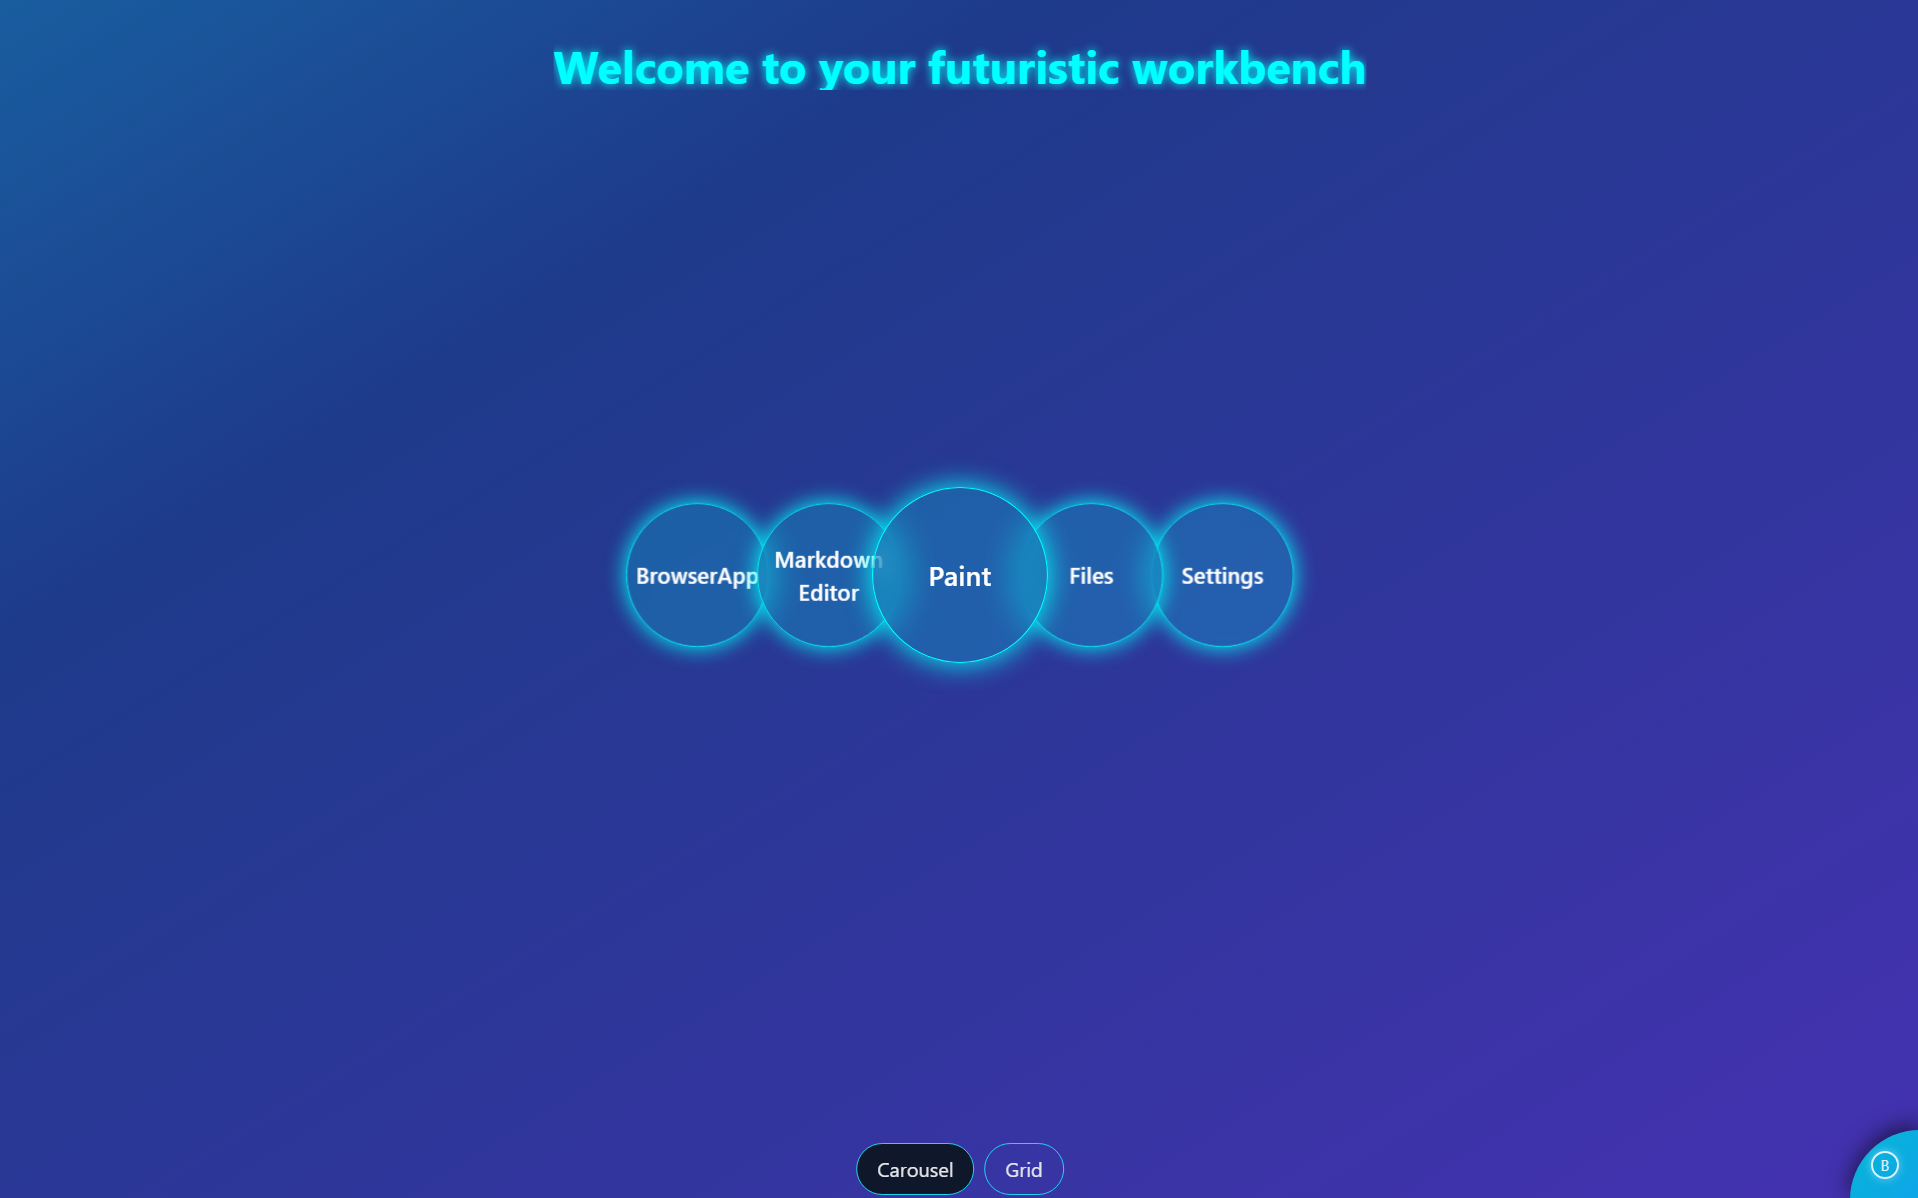
\includegraphics[width=1\textwidth]{HomeScreen.png}
  \caption{Home Screen presented to the user after start-up}
  \label{fig:HomeScreen}
\end{figure}

\newpage
\section{Specifications}
\subsection{General specifications}
% Füge hier Inhalte ein
 The “Interactive Workbench” presents an innovative and efficient System, it makes the interaction between human and machine seamless and natural. Applications like 3D-designer integrated voice assistant and more, will eliminate the need of additional monitors or the switching between Systems.
 The use case for the "Interactive Workbench" was originally only for private use. After longer development it was clear that the use case could also be spread to more public institutions like schools, maker spaces, trainings centers and so on. To meet the requirements of the user it is important to meet certain quality requirements. This can be seen in the 3D-designer and its support of mainstream formats like STL, OBJ, STEP. The overall System design which supports practicability but also appealing looks with consideration for performance. Technical  constraints as for support of all OS compatible functions and touch.
 
\subsection{Main task}
The main task of this diploma project was the development of a touch‑input‑centered, easy‑to‑use digital workbench that replaces fragmented, tool‑specific workflows with a unified digital environment for bringing ideas to life. The Interactive Workbench provides a modular user interface with several self‑developed applications that focus on intuitive gesture and touch interaction instead of classic mouse‑ and keyboard‑driven HMIs, in order to reduce time lost on portability and compatibility issues of conventional manufacturing tools. The software is implemented as a platform‑independent, open‑source web application, developed and tested using the WebStorm IDE on common desktop operating systems (Windows, macOS and Linux), so that a broad range of users can benefit from stable operation and consistent behavior across devices. A core part of the task was to design and iteratively refine the interaction concept, application architecture, and visual layout so that typical workflows around 3D‑printing and digital fabrication can be executed efficiently on a single central interface, and to validate this through practical test sessions with representative users.  

\newpage
\subsection{Technical specifications}
% Füge hier Inhalte ein
\subsubsection{Programming Languages and Frameworks}
The primary programming language used in this diploma project is JavaScript, in combination with the React framework and reusable React components. In addition, HTML and CSS are employed for structure and styling to give the workbench a clear, lively and well‑organized visual appearance. Centralized CSS style classes can be defined once and imported into multiple applications, which enables a largely uniform design language across the entire system.

For the AI assistant, Python is used because of its rich ecosystem of libraries that can be combined easily within one environment. Consequently, alongside the JavaScript‑focused toolchain (npm modules, bundler, transpiler) a Python runtime is also integrated into the development setup

\subsubsection{Target platforms}
Initially, the target platform was Linux, mainly due to its openness, compatibility and strong ecosystem for web technologies. The first prototype was therefore developed as a Linux‑only application, created without a dedicated IDE by using a simple text editor in combination with npm tooling for building and running the project.

After we discarded the Raspberry Pi 5 as primary hardware platform, the focus shifted to the software itself, which was then developed in WebStorm on two different Windows machines—a high‑performance Lenovo and a mid‑range Asus—to enable parallel work and to evaluate behaviour on different Windows setups. During a later hardware change we added a macOS installation as well, effectively turning the workbench into a cross‑platform application for Windows and macOS, with Linux remaining supported through its web‑based architecture.

\newpage
\subsubsection{Architecture}
The architecture follows a straightforward hierarchical structure. At the top we have our GUI, which, as previously mentioned, is build to guide the user through the different applications while being intuitive and easy to use. The user inputs coming from the GUI are then transferred to our backend software layer, which mainly consists of JavaScript + React applications. But before such applications are called, our software needs to identify which input has been given by the user and how to act accordingly, which is handled by our App.jsx file. That file is basically the core of our workbench, used to execute IPC events such as opening the according applications, transferring inputs to the correct applications and handling the entire backend communication. As an example, we could analyze the interaction with our AI. To communicate, the user can open a dedicated chat window, which is being opened by our main.jsx file giving the corresponding prompt to execute the jsx file for the chat window. Then, when the user sends a prompt to ollama, we use a construct of multiple files, both python and JavaScript to handle that input and deliver a clean output.  
The following block diagram displays the architecture and user input workflow used in our workbench. 
% 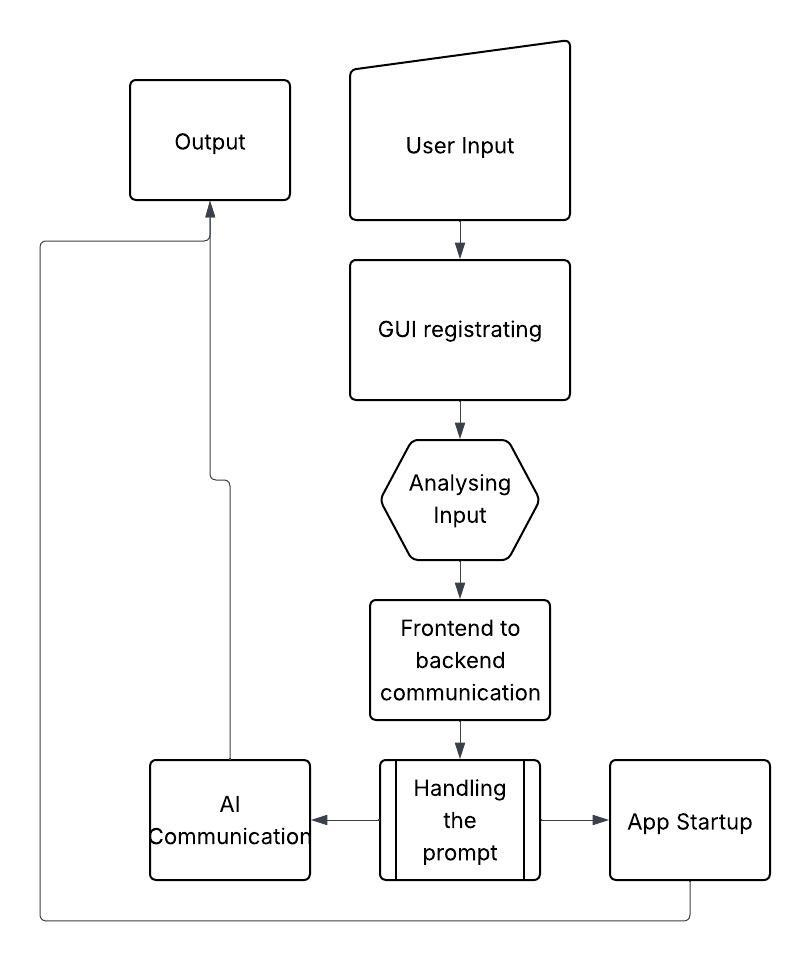
\includegraphics{User_Input_Interaction_Diagram.jpeg}
\begin{figure}[H]
  \centering
  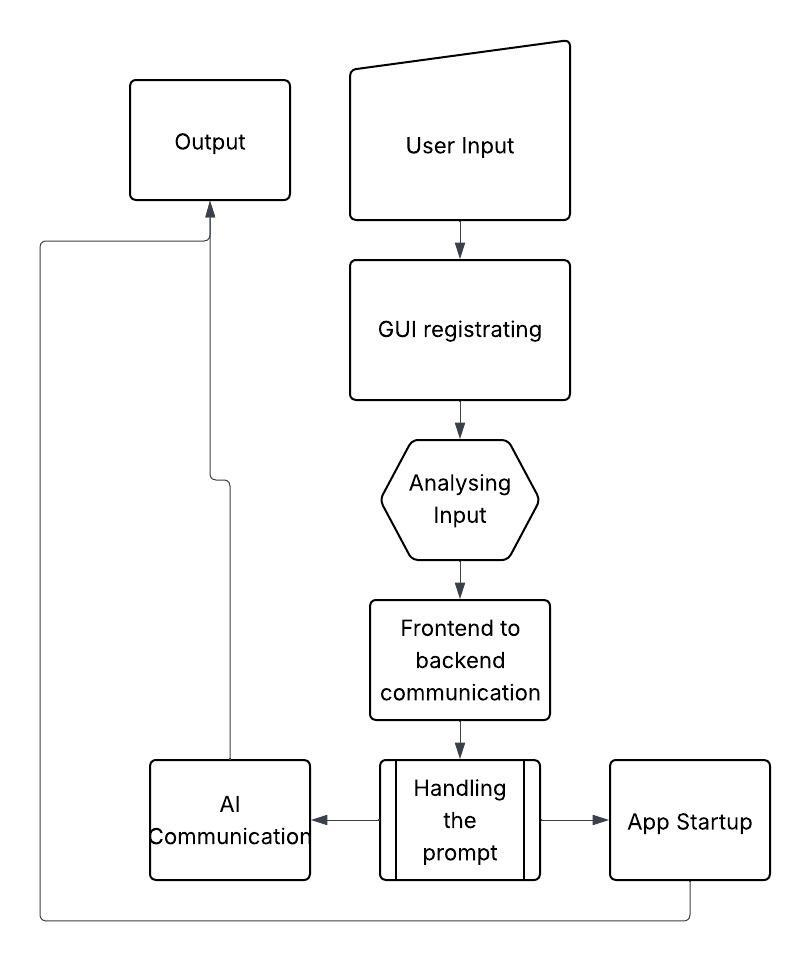
\includegraphics[width=0.6\textwidth]{User_Input_Interaction_Diagram.jpeg}
  \caption{Block diagram showing the systems architecture and input handling}
  \label{fig:blockDiagram2}
\end{figure}

\newpage
\subsubsection{Input and interaction concepts}
User interaction with the Interactive Workbench is deliberately centered on direct multi‑
touch input, complemented by full mouse and keyboard support to remain usable on any standard laptop.  The interface is optimized for finger‑based operation: large actionable areas, generous spacing and clear visuals help users recognize where interaction is possible and minimize accidental input.  A single tap (or mouse click) is used to launch applications from the home interface, confirm dialogues, and select items such as files or 3D models.

Swipe gestures are used wherever continuous navigation is required, for example to move horizontally through a carousel of applications, vertically through lists of recent projects, or to control your games.  Drag gestures extend this concept by allowing direct manipulation of on‑screen objects: in the 3D viewer, users drag to rotate the model around its axes, drag with a modifier (or two‑finger drag) to pan the camera, and combine drag with pinch‑to‑zoom to inspect fine details of a part before sending it to manufacturing.  

Within each application, the input concept follows the same principles to maintain a consistent interaction model.  Sliders and toggles are used for continuous or binary parameters (e.g. layer height or infill percentage in a printing workflow), and are dimensioned so they can be reliably adjusted with a finger rather than a mouse pointer.  Text input is kept focused and is typically restricted to clearly delimited forms, such as naming a new project or providing parameters for a task, with on‑screen and hardware keyboards supported equally.  Where appropriate, the AI assistant can be invoked via a dedicated button or command field; users then either type free‑form text prompts (e.g. “summarise the current project settings” or “suggest print parameters for PLA”) or simply ask the ai questions through voice recognition when the users hands are not free to use. Slight immediate visual feedback—through highlighting, subtle animations and status indicators—confirms that each gesture has been recognized and processed, which is particularly important when executing chains of interactions in complex workflows like preparing a print job or organizing multiple project files.

To ensure consistent touch input support across the workbench, different input concepts were evaluated for each application and component. The chosen solutions were guided by the style and usage of each application's interaction model rather than applying a one for all approach. Where continuous directional input was required, as in Byte Invaders, on-screen control buttons were introduced. Where discrete directional gestures were more natural, as in Snake, swipe detection was implemented directly on the canvas. Applications built from standard DOM elements, such as Minesweeper, required no additional work as the app's native tap-to-click mapping was sufficient. This per-application strategy ensured that touch controls felt intuitive within each context while remaining consistent with the broader interaction patterns already established throughout the workbench.

\newpage
\subsubsection{Performance and quality}
During the workbench's development, performance and quality were established as the primary evaluation criteria. The primary objective was to ensure high system responsiveness without compromising overall software quality. The development method aimed to create a balanced relationship between technical performance, usability, maintainability, and scalability rather than focusing only on speed.

Performance was evaluated from two angles. On the one hand, objective software parameters such as resource utilization, responsiveness, rendering speed, and loading times were taken into account. However, because perceived performance has a big impact on the total user experience, user satisfaction was assessed as well. Both quantifiable performance and user perception were considered because a technically quick system does not meet quality standards if it is unclear or difficult to use.

With optimization in mind, the application was created from the ground up. Modularity, component reusability, and effective state management were prioritized in the architectural choices. Hardware constraints are still important, though, especially for devices with lower performance. Because of this, the system was made to function consistently and satisfactorily across many platforms.

Since the workbench is a JavaScript-based application created with React, it benefits from a component-oriented architecture that facilitates modular development and effective rendering. React modules that had already been created and refined were incorporated to cut down on redundancy and enhance maintainability. CSS was used to implement graphic components including animations, color schemes, styles, and media assets in order to retain cross-platform compatibility and consistency while preserving performance.

\subsubsection{Compatible file formats and interfaces}
The workbench supports a variety of files. These different formats can be found and are used across many different applications of the workbench. Generally speaking, the workbench supports 3D- Files like STL, 3MF and more, used in our 3D- Viewer, the OrcaSlicer and BambuStudio. 

Considering programming languages and the available support, the workbench provides a Text- and Code editor supporting normal txt files, python files and JavaScript files. 

Our own Markdown Editor obviously supports markdown files, which can be created, edited and saved. 

Furthermore, simple apps like our paint application gives you the option to save your painting as png or jpeg files. 
These formats are also supported in our ToastUI Image Editor. 

\newpage
\subsubsection{Security and reliability}
For security reasons, the workbench is designed as a client-side focused application. All data is being processed locally on the device and is not uploaded to any external servers. This significantly reduces the risk of any unauthorized access to sensitive data, as no personal user information is required or stored. The voice input for the AI is processed locally, significantly reducing the risk of unintentionally sending requests to an external server.

For reliability the system is designed to be platform-independent, supporting all major operating systems. This ensures reliability and consistent behavior across different hardware environments. By using established programming languages such as JavaScript and libraries like React, a well tested and stability oriented user environment can be assured.

While the workbench is not intended to be used in a high-security environment, its design ensures a sufficient level of reliability and security for private or educational use cases such as, schools, home maker spaces and training centers. 
\subsubsection{Extensibility}
In terms of extensibility, the workbench provides an excellent platform. Due to its application oriented architecture, the system can easily be extended with new applications, system improvements and additional features. With this in mind, the system can be extended without requiring a complete rewrite or make major changes to the existing system, which support long term scalability. 
The use of modern and widely adopted technologies ensures future development for developers and students with a low entry barrier. For example, anyone with some knowledge of JavaScript can implement there own applications as long as there are no missing dependencies or other compatibility problems. 

% Notiz: Hier noch ein Diagramm einfügen welches das Zusammenspiel der Apps untereinander zeigt.
% -----> Wie sind App.jsy und AppCarousel.jsx etc. verlinkt.  

\subsection{Workflow: Block Diagram}
% \includegraphics{blockdiagram.png}
\begin{figure}[H]
  \centering
  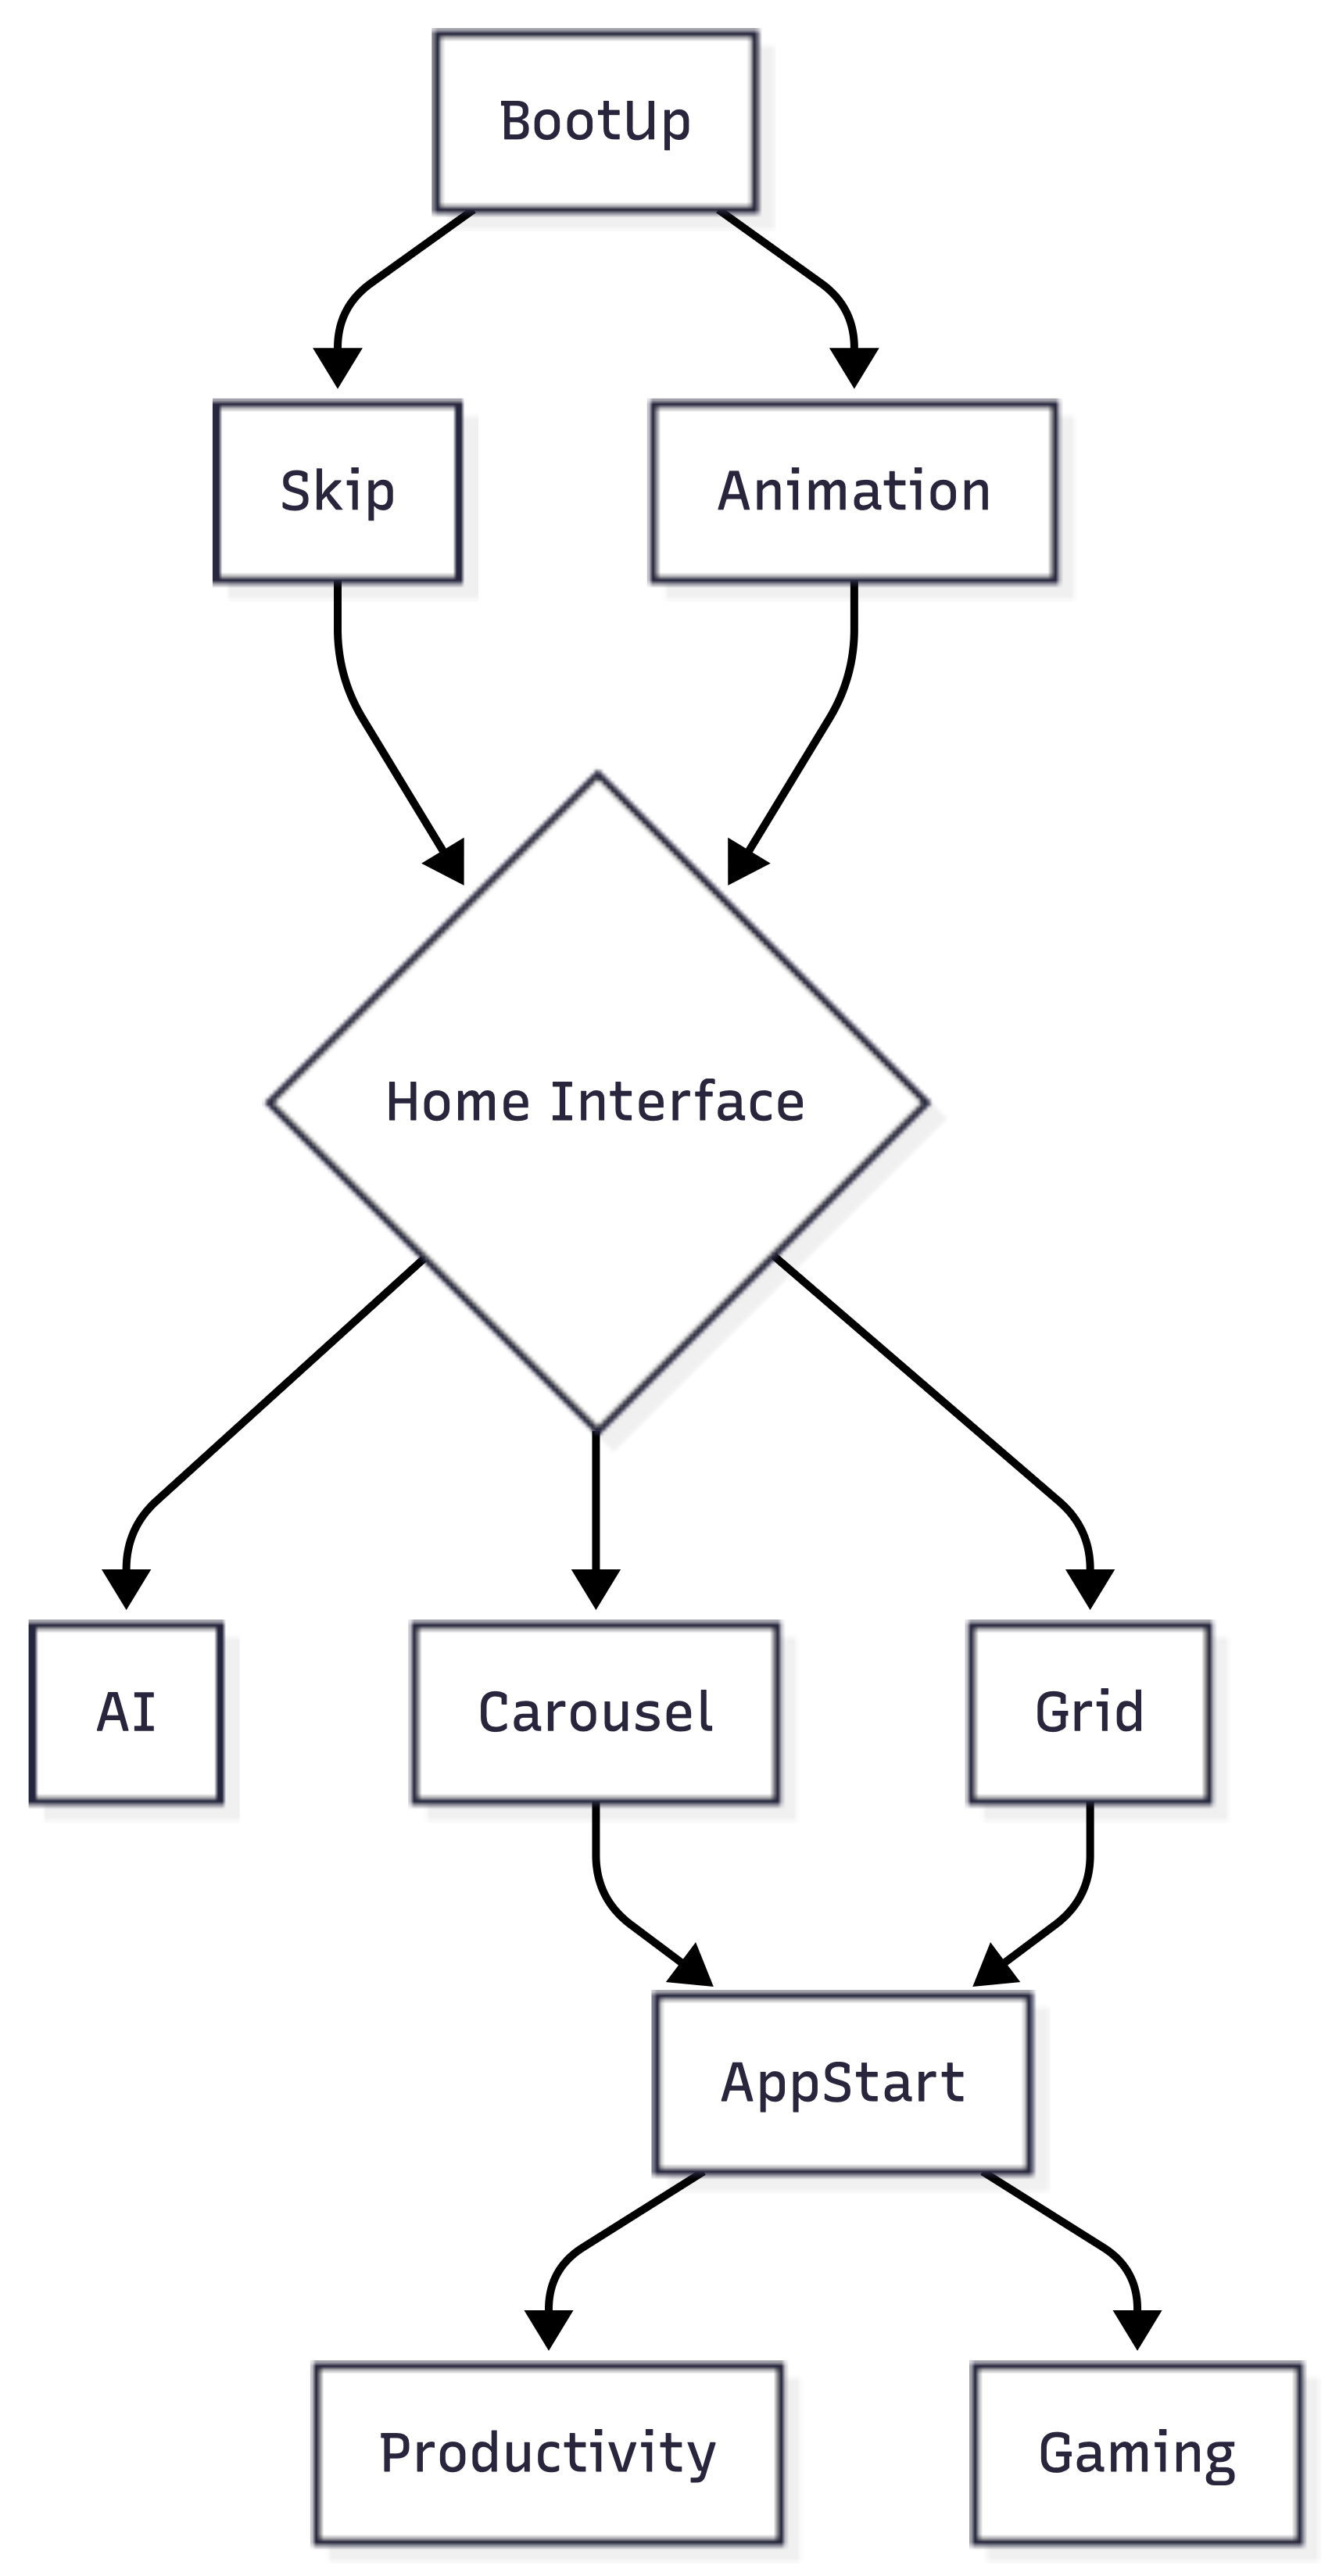
\includegraphics[width=0.6\textwidth]{BlockDiagramm.png}
  \caption{Block diagram showing the systems capabilities and workflow.}
  \label{fig:blockDiagram}
\end{figure}

This block diagram represents the systems capabilities and workflows such as its start up and the possible interactions that allow the user to access the workbenches applications, either for productivity or gaming. 

\subsection{Software requirements}
The “Interactive Workbench” can run all major operating systems. For the use of the workbench some downloads are required, as some of them are required in some applications or for the overall system. 

For JavaScript, no specific developer environment is required, making it easily accessible to users. However, certain features, such as custom application or advanced design functions, rely on additional libraries like React and Node.js/npm for local build or development purposes. Due to applications such as the 3D-Viewer the support of WebGL is required for 3D rendering. Furthermore, the React H5 Audio player was used to guarantee a well working music library. Our Image Editor requires the ToastUI Image Editor to work, which is another React Component that needs to be included when setting up the workbench. The weather application uses the API from open-meteo which not only provides the weather data but also accompany's the data with corresponding widgets which are directly used in the workbench. A complete overview of the dependencies of our project is provided by the package.json and package-log.json files, who work in a similar matter as the python requirements file. 

When it comes to python, there are multiple libraries necessary to guarantee a working chat- and voice assistant which assists you in your doing. The required libraries can be installed with the provided requirements file, which holds information about the extensions used for the assistant. Please note that, if there are two files provided, the user has to install both of these requirement files because the provided python files use different libraries to run the assistant.

Some of the applications used in the workbench are wrappers to start a 3rd- party applications. If these are missing, the workbench is not able to start these applications. These applications are BambuStudio, OrcaSlicer and FreeCAD. 

Although a specific IDE, such as WebStorm, is not required, it can simplify maintenance and help structure the code which intern helps out when working on a custom plugin for the workbench. 
If the user specifically wants to use an IDE as their primary target is to extend the workbenches capabilities, we can highly recommend WebStorm, using it under the non-commercial license.  

This does not mean that other IDEs are not able to run the project or offer a nice GUI to work with, we prefer WebStorm. 
% Füge hier Inhalte ein
\newpage
\section{Project planning}
\subsection{Division of tasks}
Given the scope and complexity of the diploma project, a structured division of responsibilities was essential to ensure efficient collaboration and balanced workload distribution. From the beginning, tasks were clearly assigned in accordance with each developer’s strengths and the project’s technical requirements.

GitHub served as the central collaboration platform, supporting version control, documentation, and transparent task tracking. All planned features were documented with sufficient detail to establish a shared understanding of objectives and implementation requirements.

While responsibilities were clearly distributed, certain complex components required joint development. In these cases, both developers collaborated on architectural design, implementation, and refinement. This cooperative approach ensured technical consistency across modules and supported knowledge exchange throughout the development process.

The structured allocation of responsibilities contributed significantly to steady progress and minimized coordination overhead.

\begin{figure}[H]
  \centering
  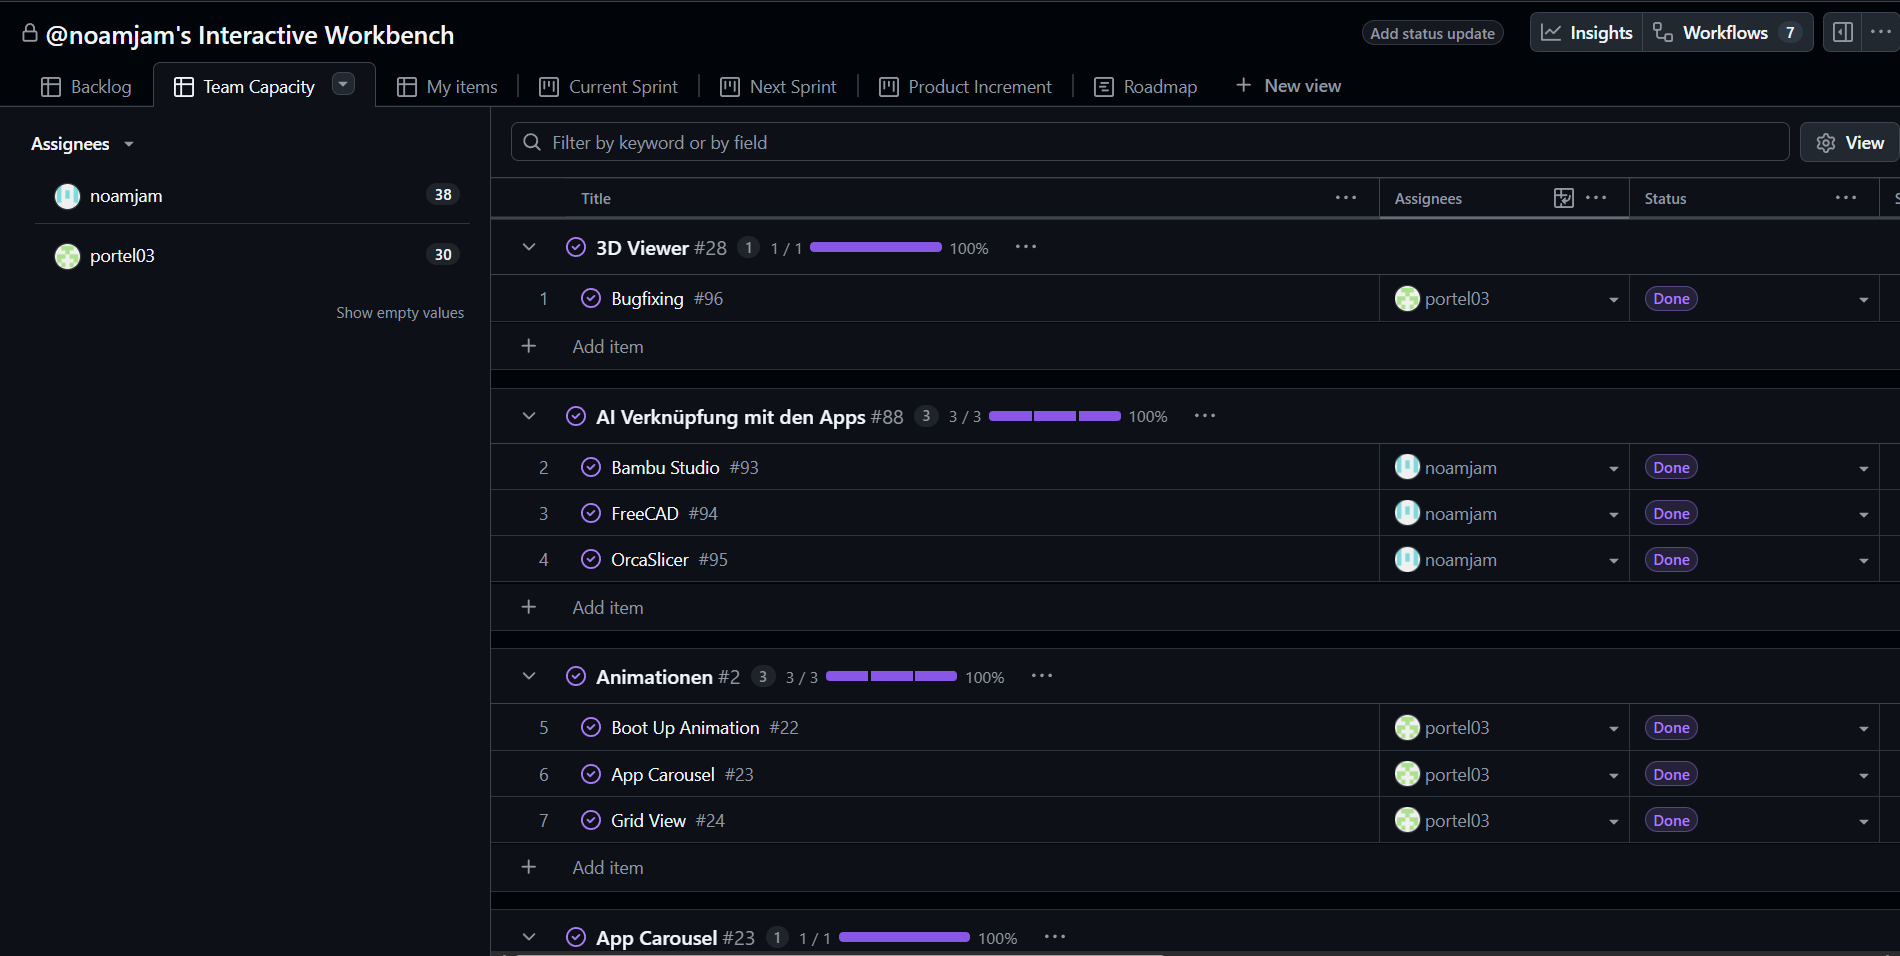
\includegraphics[width=1\textwidth]{Division_of_tasks.png}
  \caption{Team capacity and division of tasks.}
  \label{fig:Team capacity}
\end{figure}


\newpage
\subsection{Solutions and development planning}
\subsubsection{Solutions}
To realize the vision of a user-friendly, stable, and secure graphical user interface, several technological and architectural decisions were evaluated during the initial design phase. The selection of tools and frameworks was guided by criteria such as platform independence, scalability, maintainability, and data security.

JavaScript was selected as the primary development language due to its suitability for web-based applications and its broad cross-platform compatibility. As a browser-supported technology that also enables local desktop application development when combined with React, it enables platform-independent deployment without system-specific adaptations. This ensures consistent functionality across devices while maintaining architectural flexibility.
The workbench was implemented using React to establish a component-based architecture. This model promotes modular development, reusability, and a clear separation of concerns. By structuring the system into independent yet interconnected components, future extensions and modifications can be implemented without fundamental restructuring.

Data security and privacy were addressed through a local-first architecture. All processing tasks — including AI-related computations — are executed locally on the user’s device, and no sensitive data is transmitted to external servers. This approach enhances transparency, reduces latency, and strengthens user trust.

Overall, the chosen technology stack provides a sustainable and scalable foundation for achieving usability, stability, and long-term maintainability.

\subsubsection{Development planning}
The development planning phase established the methodological and structural foundation of the project. Due to the technical scope of the workbench — including AI integration, 3D visualization, and the consolidation of multiple applications within a unified graphical user interface — a systematic and forward-looking planning strategy was required from the outset.

The project originated as a private prototype developed during the summer. After evaluating its technical potential and practical relevance, the concept was formalized and submitted as the official diploma project. Following approval at the end of September, the development process was aligned with clearly defined objectives, architectural guidelines, and academic requirements.

An agile development methodology based on Scrum principles was chosen to ensure flexibility and continuous refinement. Rather than relying on rigid long-term planning, the project was structured into iterative cycles, enabling progressive implementation and regular evaluation of intermediate results. This approach ensured steady progress while allowing adaptation to technical challenges and evolving requirements.

Development planning therefore combined strategic foresight with iterative execution, forming the organizational backbone for the subsequent technical implementation.

\newpage
\subsection{Scheduling}
The scheduling of the project was closely aligned with the chosen agile methodology. After the project was officially approved at the end of September, development efforts were intensified and organized into weekly iterations.

Each development cycle included task definition, implementation, and a review phase in which completed features were evaluated and, if necessary, revised in subsequent iterations. This iterative structure enabled continuous system improvement and ensured that emerging challenges could be addressed promptly.

Early scheduling focused on foundational and technically demanding components, such as AI integration and the 3D viewer, as these elements significantly influenced the overall system architecture. Prioritizing these features reduced architectural risks and created a stable basis for subsequent modules.

Major milestones included the public presentation of the first functional prototype during the school’s open day. At the present stage, the technical development of the workbench is largely complete, and the primary focus has shifted to the documentation and finalization of the diploma thesis.

The scheduling strategy thus ensured structured progress, milestone-oriented development, and adaptability throughout the project life cycle.% Gantt-Chart oder Tabelle einfügen

\begin{figure}[H]
  \centering
  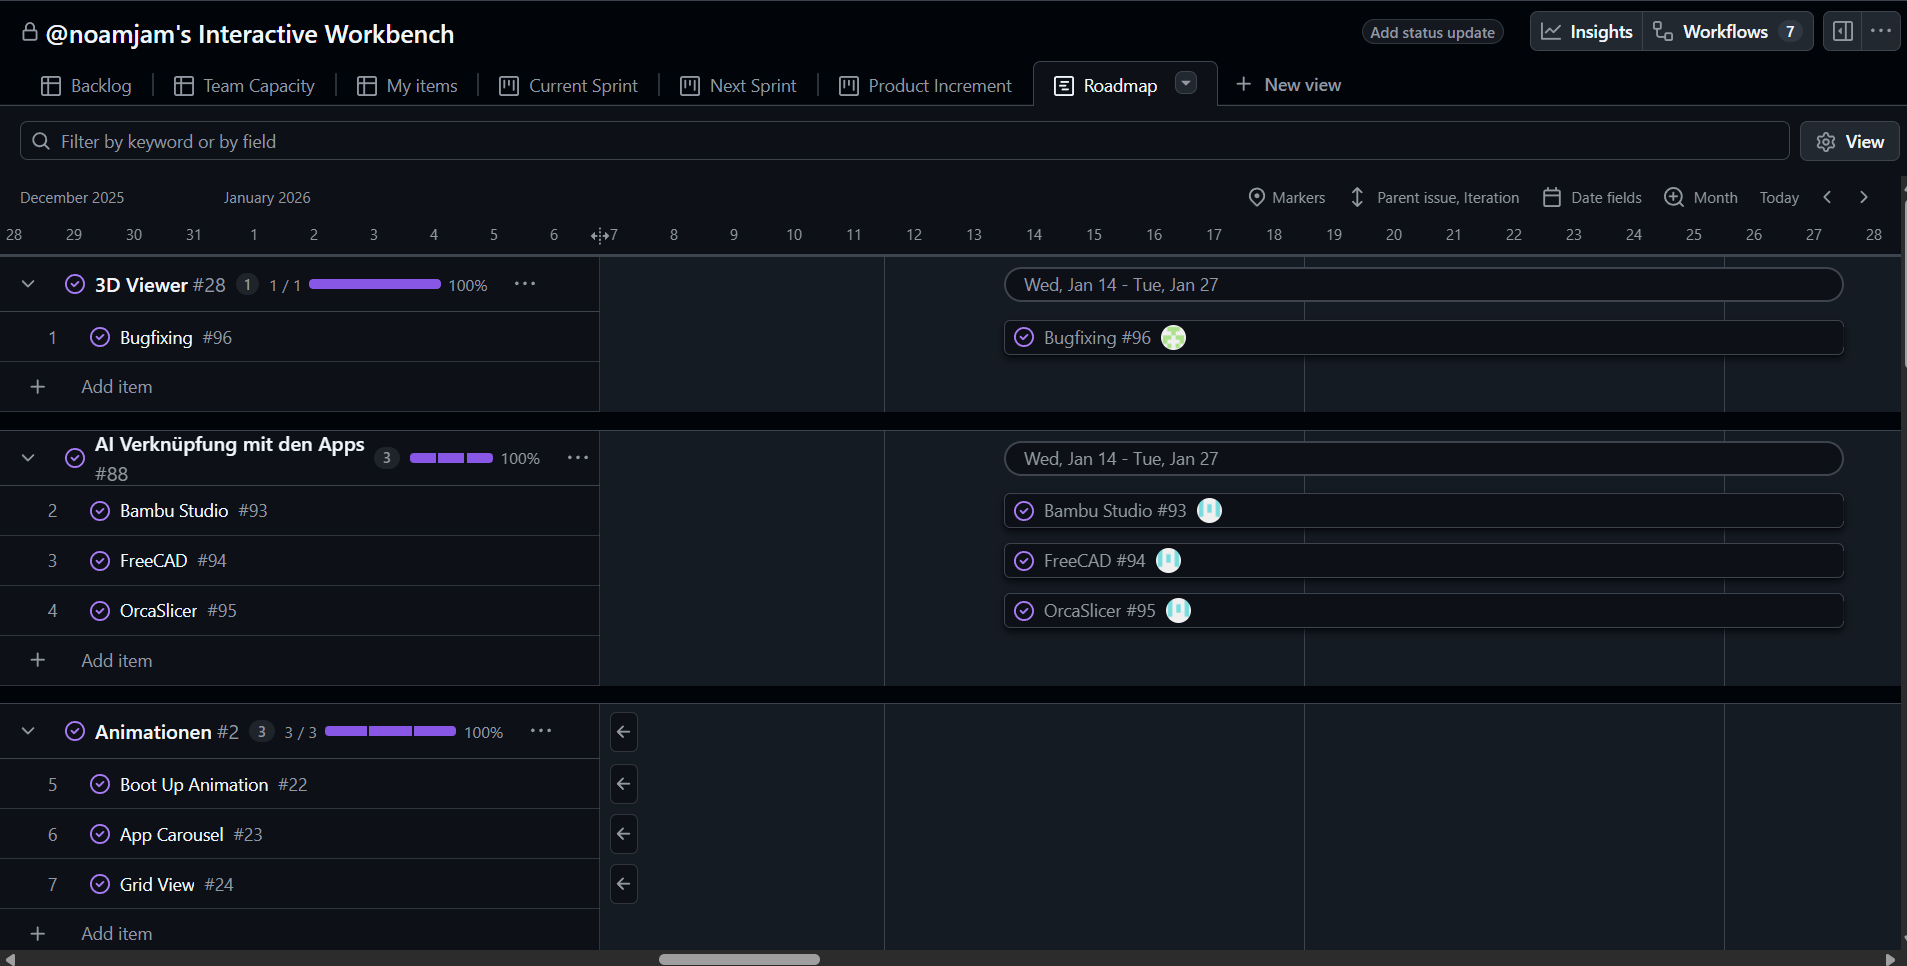
\includegraphics[width=1\textwidth]{Example_GitHub_Roadmap.png}
  \caption{GitHub Development Roadmap.}
  \label{fig:Roadmap}
\end{figure}


\newpage
\section{Project realization and software development}
The software development in the given time period was based on a prototype, previously developed by us. That prototype didn't have any function and was a raw model of our GUI. Build in a Virtual Machine running a Linux distribution, we started out by making a windows port which was relatively easy thanks to the flexibility of WebStorm, our IDE of choice. 
The prototype was developed with extensibility and compatibility in mind. 

\subsection{Backend software development}
This section describes the not only the functionality but also the technical side of our applications and software offered by our workbench. 
This section will be structured according to but not limited to the core applications of our workbench. 

\subsubsection{Paint}
\paragraph{First iteration} \mbox{} \\
The first iteration introduced a simple version of a paint application which allowed the user to draw out there imagination using either touch input or with a mouse. 
The software was engineered using JavaScript and React. To put it simply, the canvas recognizes user inputs, follows movement and places a line at the according coordinates. 

\paragraph{Interaction concepts and technical functionality}
\subparagraph{Interaction model}\mbox{} \\
The application is based on the HTML5 canvas element and implements a real-time drawing system using event-driven interaction. User input is captured through both mouse and touch events, ensuring compatibility across desktop and touch-enabled devices. By supporting mousedown, mousemove, and mouseup events as well as their touch equivalents, the system enables continuous and platform-independent drawing interaction.

The drawing logic differentiates between three operational modes: freehand drawing, straight line rendering, and circle creation. Freehand drawing is implemented as a continuous stroke process, where successive cursor positions are connected dynamically to form smooth lines. In contrast, geometric shapes are defined by an initial starting coordinate and a final endpoint, from which dimensions such as length or radius are calculated before rendering.

This distinction between continuous and parameter-based drawing modes allows intuitive interaction while maintaining a clear internal logic structure.

\newpage
\subparagraph{State management and rendering logic}\mbox{} \\
The application utilizes React’s state management mechanisms to control drawing behavior, tool selection, color configuration, and stroke width. Dynamic updates to these parameters are reflected immediately in the canvas rendering context, ensuring responsive user feedback.

The rendering process itself is handled directly through the 2D drawing context of the canvas element. Line smoothing is achieved by configuring rounded line caps and joins, improving visual quality and user experience. Canvas dimensions are programmatically synchronized with the rendered element size to prevent scaling distortions.

\subparagraph{Undo and redo mechanism} \mbox{} \\
A notable technical feature of the application is the implementation of an undo/redo system. Instead of storing individual drawing commands, the application captures complete canvas states as encoded image data after each finalized drawing action.

These snapshots are stored in a history stack, enabling backward navigation through previous states. When an undo operation is triggered, the most recent state is removed and the preceding image is re-rendered onto the canvas. A complementary redo stack allows restoration of reverted states.

While this approach increases memory usage compared to vector-based storage, it simplifies state restoration and ensures reliable behavior across different drawing modes.

\subparagraph{Additional functional features}\mbox{} \\
The application includes supplementary usability functions such as:
\begin{itemize}
    \item Dynamic color selection
    \item Adjustable stroke thickness
    \item Canvas clearing
    \item Export the final drawing as a PNG image file
\end{itemize}

The export functionality converts the current canvas content into a Base64-encoded image and triggers a client-side download process. All operations are executed locally within the workbench environment, ensuring independence from external services.

\paragraph{Architectural design}\mbox{} \\
The architecture of the paint application is simple as it only consists of the canvas in which the user can draw, the toolbar and the communication between both of these things and the JavaScript functions as well as the HTML/CSS styling. 
\newpage
\paragraph{Iterative refinement}\mbox{} \\
During its development, the paint application underwent several iterative refinements. The initial version provided only basic freehand drawing functionality and served primarily as a proof of concept for canvas-based rendering within the workbench environment. In a subsequent iteration, the application was extended with a structured toolbar, tool selection options, and improved rendering behavior, resulting in a significantly smoother and more user-friendly interaction experience.

At a later stage, an attempt was made to further optimize drawing performance, particularly for direct touch input on touchscreen devices. The objective was to improve stroke smoothness and responsiveness by introducing alternative event-handling mechanisms. However, the intended implementation relied on event-handling approaches that were not fully supported within the chosen JavaScript environment and application context. This resulted in instability and inconsistent drawing behavior.

Due to these technical constraints, the optimization attempt was discontinued, and the application architecture was reverted to the previously stable version. Although this version did not achieve the desired level of stroke smoothness under all touch conditions, it provided reliable and predictable behavior across devices. The decision to prioritize stability over experimental optimization reflects a broader development principle applied throughout the project.

\newpage
\paragraph{Current limitations}\mbox{} \\
The application is currently limited by JavaScript and React itself. To our knowledge, there is no current methodology that supports faster inputs and smoother drawings. 
It could be improved with newer versions of React. 

\begin{figure}[H]
  \centering
  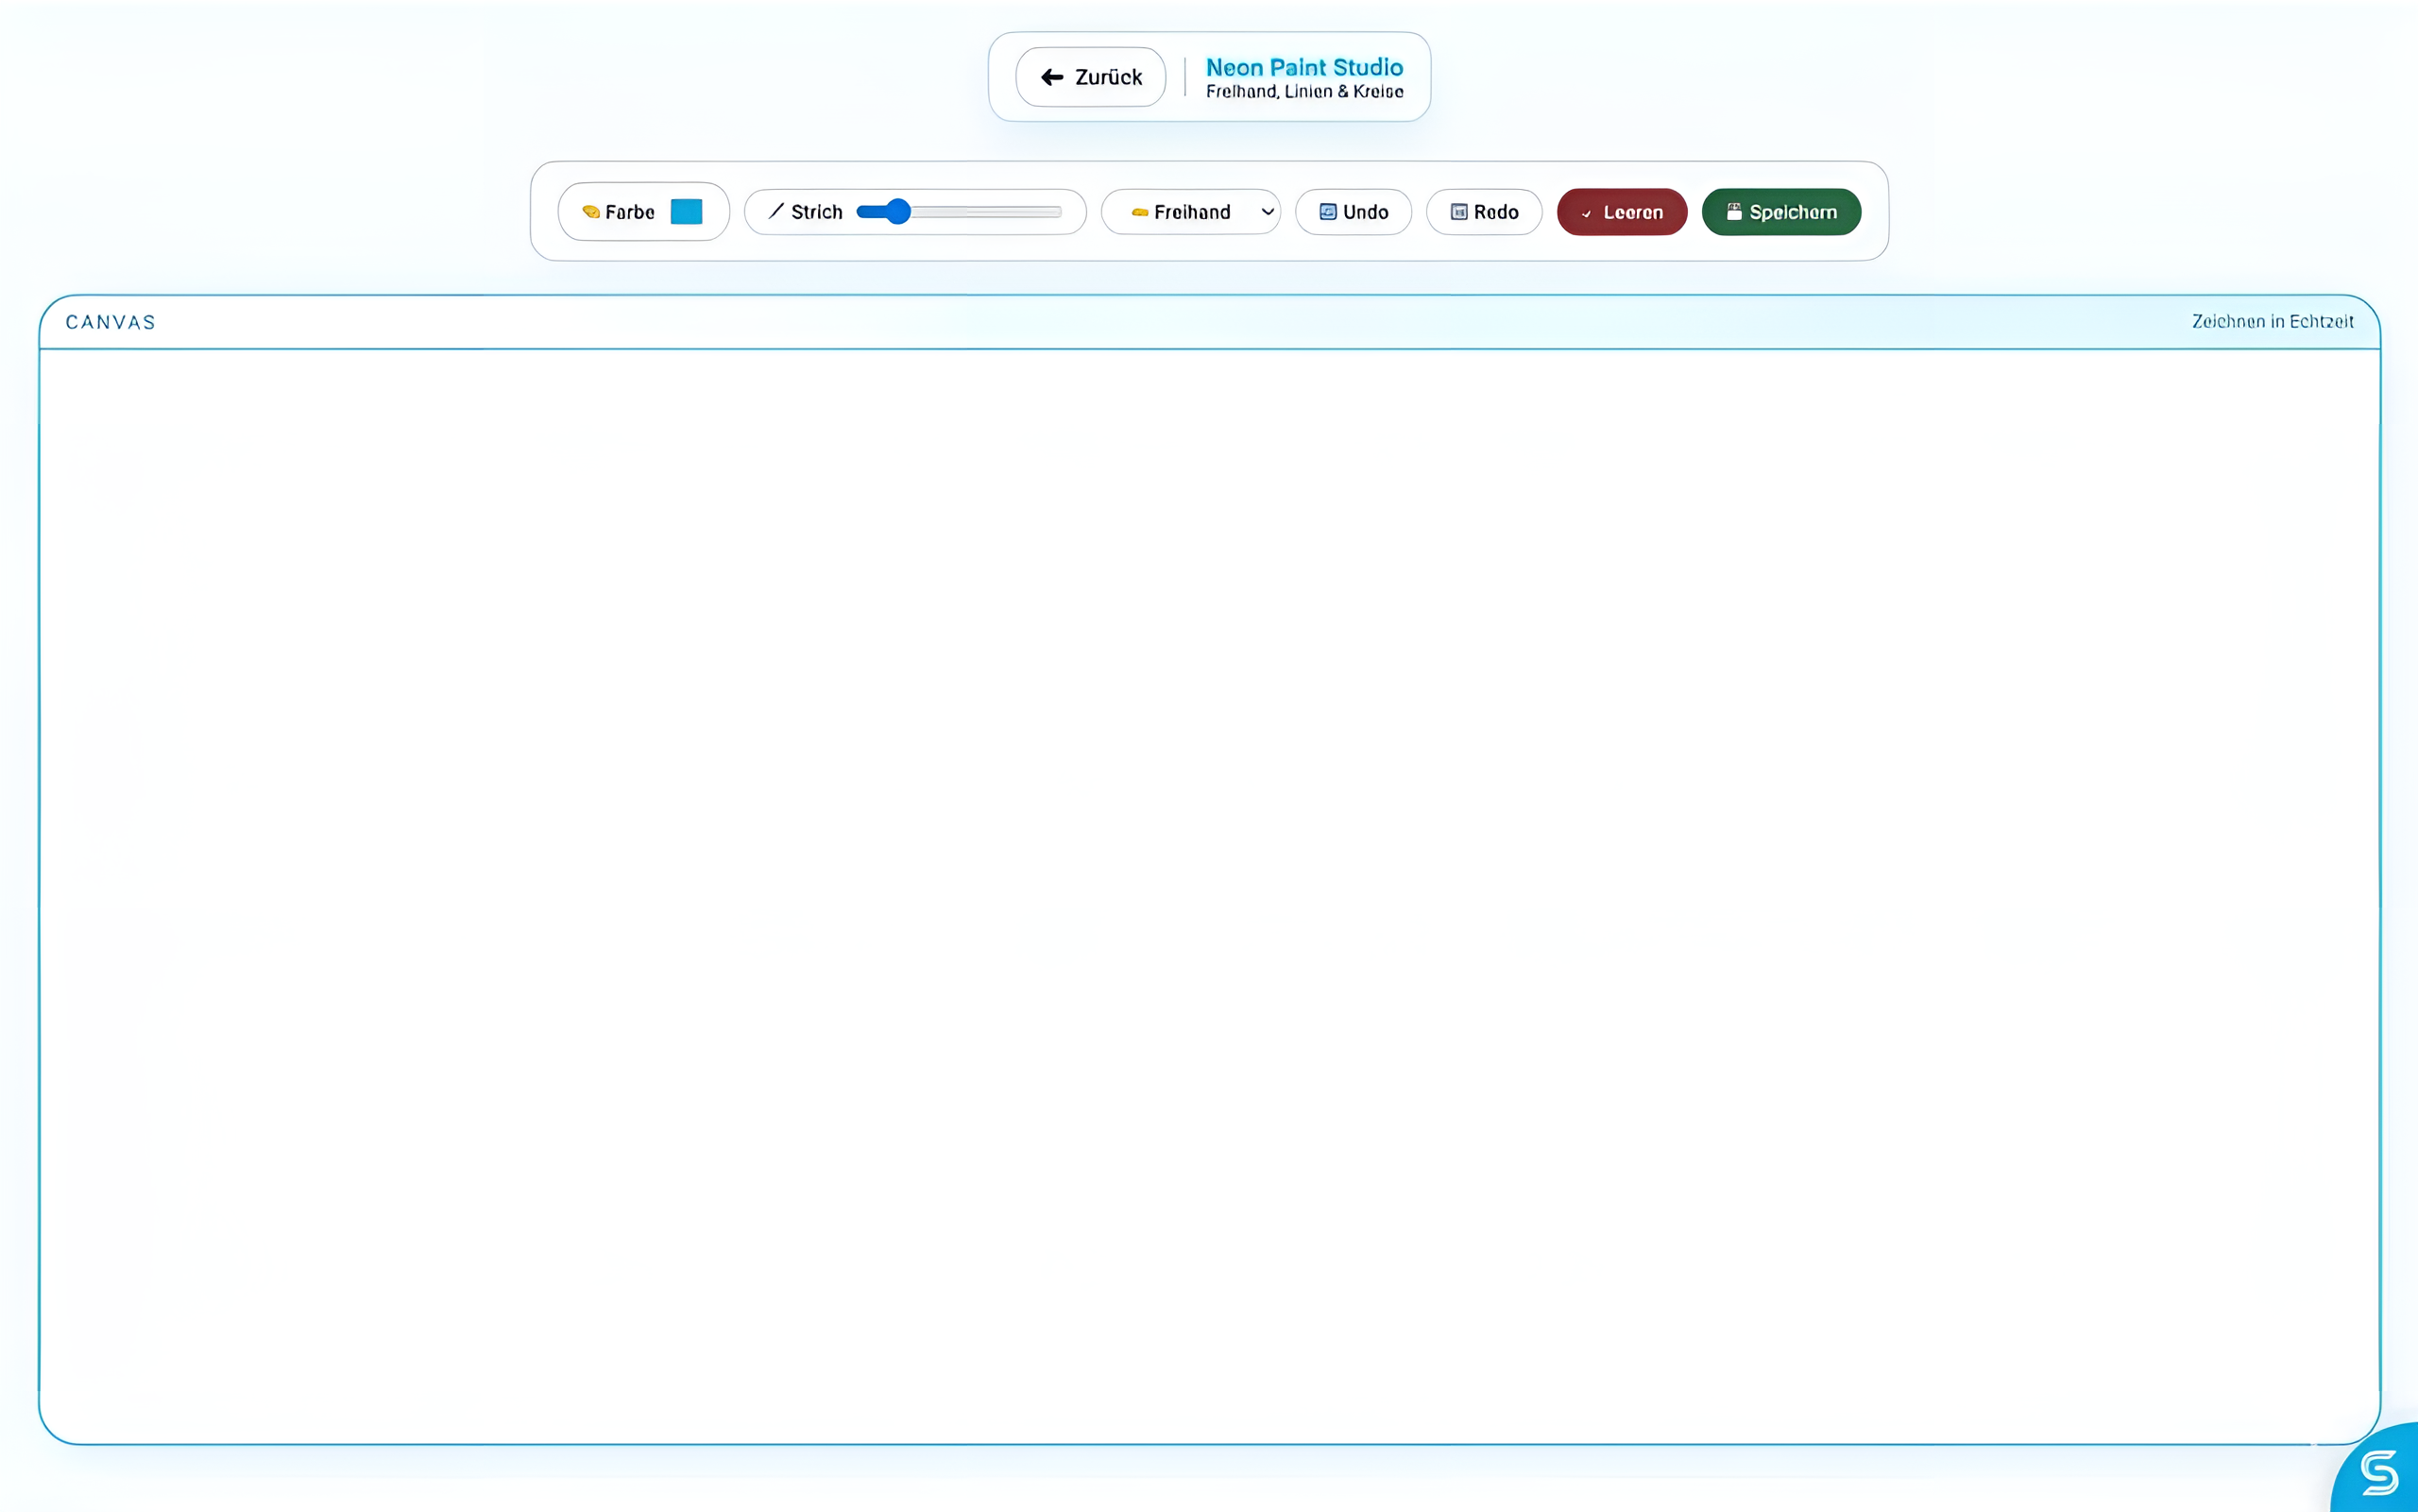
\includegraphics[width=1\textwidth]{Paint.png}
  \caption{Paint application- converted to white background}
  \label{fig:Paint}
\end{figure}

\newpage
\subsubsection{AI development}
\paragraph{AI Processing Module}\mbox{} \\
The AI assistant represents one of the central backend components of the workbench. While its functional purpose and integration into the GUI have been described in previous sections, this chapter aims specifically at the development side and the technical implementation and architectural structure of the AI assistant. 

\paragraph{Architectural design}\mbox{} \\
The AI module was implemented as a locally executed Python- based process, technical separated from the JavaScript frontend environment, but still ready to use at the click of a button. 
The separation between the JavaScript frontend and the python backend was chosen to ensure modularity, maintainability, and independence from rendering layers. This helped make the workbench more stable as a complete system and also preserve responsiveness. 

Communication between the frontend and the AI backend is handled through a structured interface layer. User input entered in the GUI is transferred to the python process, where it is processed and interpreted before the generated response is returned to the frontend for visualization. This bidirectional communication required careful synchronization to avoid execution conflicts and response delays. 

At its current state, the AI- chat can be opened in separate React applications, which first simplifies the user input and transfers it to the python- backend which then uses WebSocket communication and FastAPI to send the user input to the users local IP- address in combination with the port that the users local LLM of choice runs on and give it back to the GUI. This is accompanied by a simple but effective status handling logic which provides debug information such as "active, thinking, standby". 

Furthermore, the AI assistant can also be interacted with using voice commands. This requires a specific trigger word to be spoken. Once active, the assistant will listen and stand ready to answer the users prompts until the user tells it to go into standby mode with another trigger word. This is achieved by analyzing the user input and search it for these trigger words. In detail, the audio part is handled by the python "pyaudio" library, while the text to speech translation is handled by Googles "gTTs" service, also running locally on the users device using python. 

A part of its architecture is that it is able to interact with other components of the workbench and its applications. 

\newpage
\paragraph{Iterative refinement}\mbox{} \\
The AI assistant underwent substantial conceptual and architectural evolution during the course of development. In its earliest state, it functioned exclusively as a voice assistant understanding basic prompts but only to a certain extend. User input was limited to speech only, which was forwarded and processed by a LLM of the users choice, in our case ollama, before generating a response text which was then played auditory using python. While this implementation successfully demonstrated local speech recognition and model connectivity, it lacked flexibility and offered no alternative interaction modality as well as being slow, tiring to work with and not the best at understand user inputs. 

A major refinement occurred with the introduction of a text-based chat interface. This addition transformed the assistant from a purely voice- driven feature into a hybrid communication system. Text input significantly improved accessibility and debugging efficiency, as prompts could now be entered and tested directly without relying on microphone input. This shift also improved reliability in situations where speech recognition produced inconsistent results. Conceptually, the assistant evolved from a voice utility into a fully integrated communication module within the workbench. This also came with the benefit of being able to return to previous chats with the ai as the chat- interface would only clear out on the users command or when shutting down the workbench. The methodology of text- based answers also introduced a lot of practical features like the option to copy and paste ai generated code directly from the chat- interface into the workbenches own text and code editor. 

Parallel to these interface changes, the backend architecture matured considerably. The assistant was restructured into a modular system consisting of a FastAPI backend for model communication, an Electron main process for orchestration, and a React-based frontend for visualization. Stability improvements were implemented after encountering issues such as incorrect timeout configurations, which previously caused server crashes during model requests. Correct handling of asynchronous HTTP requests and proper timeout definitions significantly improved robustness and eliminated recurring 500-level errors.

\newpage
The most significant conceptual expansion occurred when the assistant was connected directly to  other applications in the workbench. A command bridge was introduced between the Python backend and the Electron main process. On the backend side, a structured Command model was implemented to allow the assistant to return both a natural language reply and an optional executable instruction. User prompts were scanned for defined trigger keywords, and if detected, a corresponding command object was attached to the response. On the Electron side, an IPC handler processed these commands and, after explicit user confirmation, launched other programs through secure child process spawning. 

Through this mechanism, the assistant gained the ability to open applications such as FreeCAD, Bambu Studio, and OrcaSlicer directly at the user’s request. This functionality required coordinated development across multiple layers of the system, including Python-based command generation, JSON serialization of tool instructions, IPC communication, and platform-dependent process handling in the main process. The integration demonstrates a shift from passive text generation to actionable system control, effectively turning the assistant into a lightweight orchestration layer within the workbench.

Overall, the AI assistant evolved from a voice-only experimental feature into a modular, hybrid interaction and control system. The iterative refinements reflect not only technical improvements in stability and architecture but also a gradual expansion of scope — from answering questions to executing commands and interacting with the broader software environment. This progression illustrates a clear transition from prototype functionality toward a robust and extensible subsystem integrated deeply into the workbench ecosystem.

\newpage
\paragraph{Current limitations}\mbox{} \\
The biggest limitation to the performance to the ai is something that we value just as much as performance, and that is security. As a consequent of running everything locally on the users device, we lose a lot of performance as the LLM can take up to about 5GB of RAM. This means that, on lower end machines, if the ai runs, it will run relatively slow. 
On the other hand, assured this approach a higher level of security and safety. Another limiting factor is cost. Using well performing models with a high count of parameters, not only consumes more hardware, but is also expensive because of licensing costs. 

Another problem is that to set up the assistant in the first place, a stable internet connection is required. 

\begin{figure}[H]
  \centering
  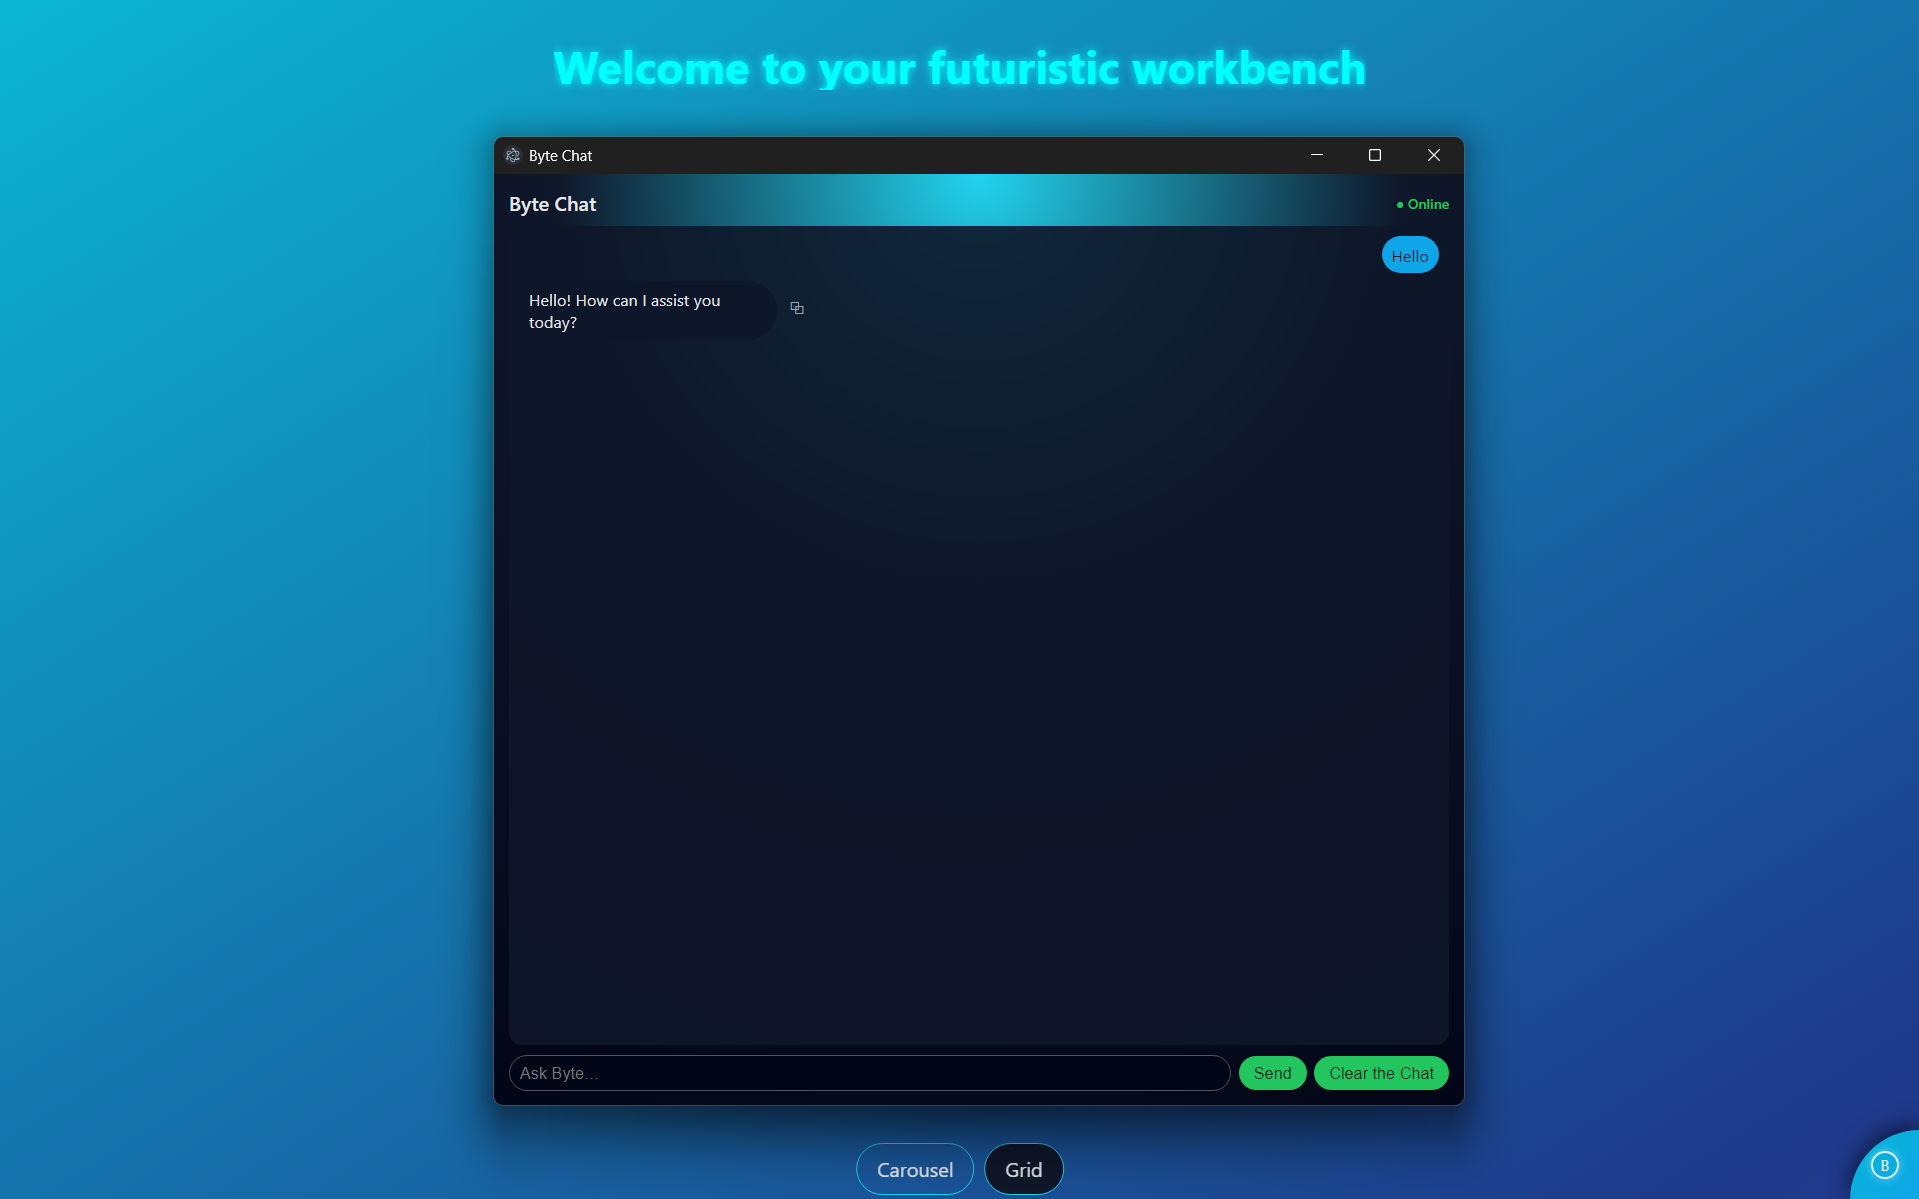
\includegraphics[width=1\textwidth]{byte_assistant.png}
  \caption{AI- Assistant: byte assistant}
  \label{fig:AI}
\end{figure}

\newpage
\subsubsection{Text and code editor}
This section will introduce you to the text and code editor on a deeper and more technical level. We will cover its development as well as its functionality. 

\paragraph{Initial implementation and functional scope}\mbox{} \\
Initially, the text and code editor was introduced as an independent productivity application within the workbench. In its first state the component provided basic text editing functionality, allowing the user to create and modify plain text within a structured graphical interface. The primary objective at this stage was the interface integration and consistency with the overall visual and interaction design of the workbench. 

Early development focused on usability, responsiveness, and seamless embedding into the central GUI architecture. The editor was designed to operate as a self- contained module while maintaining 
compatibility with the navigation and application-switching logic of the workbench, like for example, using the ai to generate text and then paste it into the editor. 

Over the course of development, the scope expanded and the support offered by the application went from simple text manipulation towards a structured development- oriented editor capable of supporting simple programming workflows. 

\newpage
\paragraph{Iterative refinement}
\subparagraph{Extensions to code-oriented functionality}\mbox{} \\
The transition from a plain text editor to a functional code editor marked a significant refinement stage. The application was extended to support structured code input for multiple programming languages, specifically Python and JavaScript. This extension required not only frontend improvements but also backend-level integration to enable actual code execution.

The editor interface was enhanced to clearly separate input and output areas, enabling users to write code and directly observe execution results. This refinement transformed the application from a passive writing tool into an interactive development environment embedded within the workbench.

The applications styling underwent a serious overhaul. We changed the layout, colors and animations. A newly added sidebar now worked as a simple file explorer hub, so the user gets a better view of current files and projects. 
We also added some buttons which brought with them a lot of functionality. 

This iteration introduced functionalities such as file creation, deletion, closing and opening in the explorer hub and form the file system, a run button to execute code and syntax highlighting. 
The syntax highlighting was achieved using the React Monaco-Code-Editor integration. 

The shift illustrates a conceptual evolution: instead of merely hosting static utilities, the workbench began to integrate active runtime capabilities.


\subparagraph{Backend execution architecture and coding language support}\mbox{} \\
A central architectural milestone was the implementation of a dedicated execution endpoint within the Electron main process. When users request code execution, the frontend transmits the code and selected language to the backend, where a child process is spawned using the appropriate interpreter.

Interpreter selection is handled dynamically depending on the operating system and programming language. For Python execution, the system selects either python or python3 depending on platform conventions. For JavaScript, a Node.js runtime is invoked. This abstraction ensures cross-platform compatibility while maintaining a unified execution interface.

The execution process is isolated from the renderer process, preserving application stability even in cases of runtime errors. Output streams (stdout and stderr) are captured and merged before being returned to the frontend for structured display.

This separation between interface and execution logic reinforces modularity and prevents frontend instability from propagating into system-level operations.

\newpage
\paragraph{Stability, safety, and resource control}\mbox{} \\
Allowing arbitrary code execution within a desktop environment introduces potential risks regarding performance and system integrity. To address these concerns, multiple control mechanisms were implemented.
Execution time is limited through a defined timeout mechanism. If a process exceeds the allowed runtime, it is terminated automatically. Additionally, output size is restricted to prevent excessive memory usage caused by large print statements or infinite loops. These safeguards ensure predictable system behavior even under unintended or erroneous code conditions.
Error handling was refined to return structured and informative responses instead of generic crashes. Interpreter launch failures, missing runtime environments, unsupported language selections, or runtime exceptions are captured and displayed transparently in the output panel. This approach improves reliability and provides meaningful feedback to the user.
Through these measures, the editor balances flexibility with operational safety.

\paragraph{Current limitations}\mbox{} \\
At its current state, there are limitations to what the Editor can do. As previously mentioned, we but a lot of thought into resource control because the workbench as it is requires resources that some devices don't have. Combine that with things like the locally running LLM, you end up with a high level of stress for your hardware. So we opted to go for things like limited execution time and such. This means that a conversion to a full on IDE is highly doubtable as that would not only require a tremendous amount of time but also resources. Language support is also something to think about, because the currently supported languages, python and JavaScript have been explicitly chosen by us as they are the main languages in use in our workbench. 

\begin{figure}[H]
  \centering
  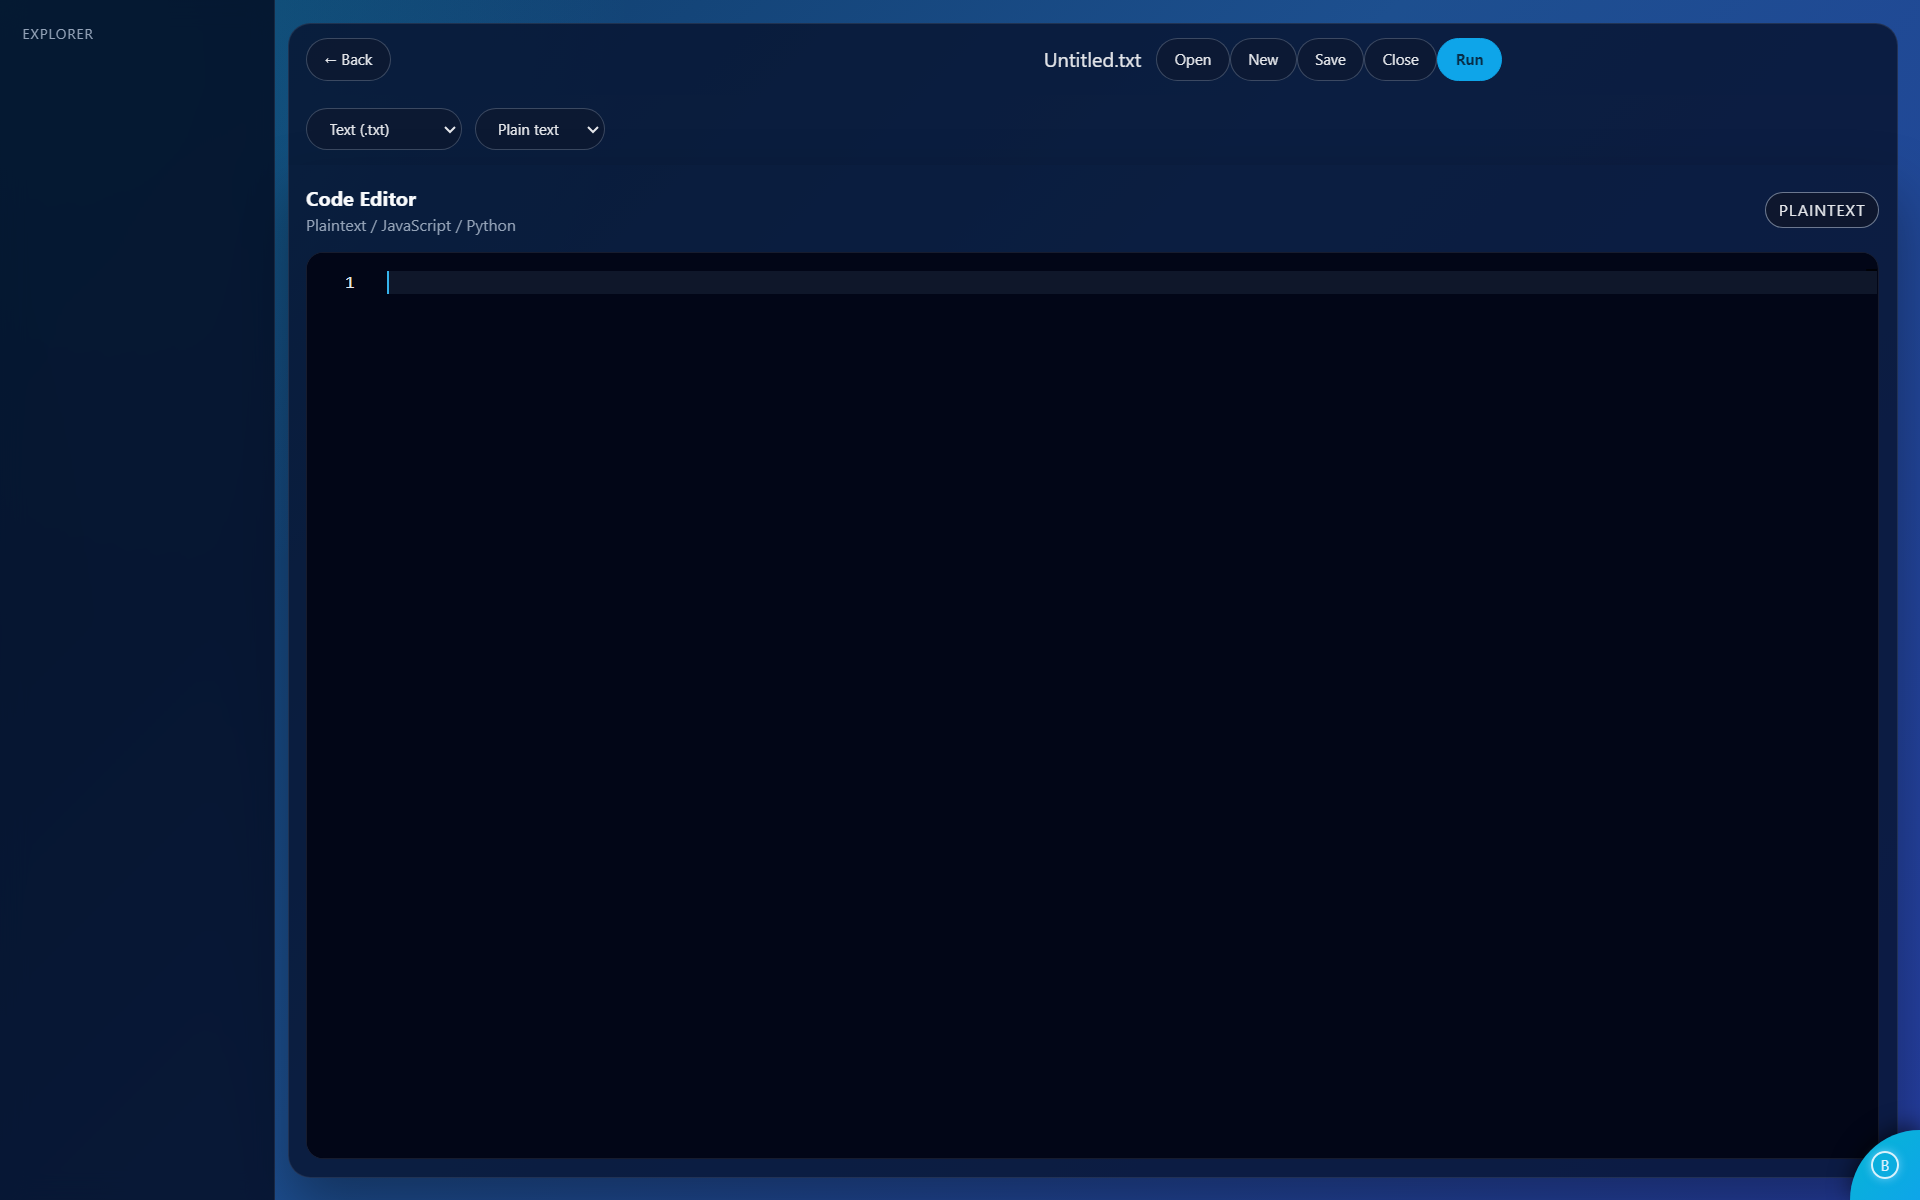
\includegraphics[width=0.9\textwidth]{IDE.png}
  \caption{Text- and Code- Editor}
  \label{fig:IDE and plain text editor}
\end{figure}

\subsubsection{Markdown editor}
This section introduces the Markdown Editor and discusses its development, architectural integration, and functional capabilities within the workbench environment. The application was designed to provide a lightweight documentation and note-taking tool that integrates seamlessly with the workbench's graphical interface and application ecosystem. 

The primary goal of the editor was to enable structured documentation using Markdown syntax while maintaining the interactive design philosophy of the workbench. In contrast to the text and code editor, which focuses on general writing and code execution, the Markdown editor specifically targets structured documentation workflows such as note-taking, documentation writing, and quick formatting of technical content.

\paragraph{Initial implementation and integration into the workbench}\mbox{} \\
The Markdown editor was introduced as a dedicated application inside the workbench’s application carousel. Similar to other applications within the system, it can be launched through the central navigation interface where each application is represented as a selectable tile.

When the Markdown editor is selected, the main application state changes to render the Markdown editor interface as an overlay component within the Electron renderer process. This design follows the same architectural pattern used by other workbench applications, ensuring consistency in navigation behavior and window management.

At this stage of development, the main objective was to integrate a functional editing interface capable of handling Markdown formatted text while maintaining compatibility with the workbench’s existing React-based GUI structure. The editor was therefore implemented as a modular component that communicates with the main application state while remaining functionally independent.

\paragraph{Iterative refinement}
\subparagraph{Editor interface and live preview architecture}\mbox{} \\
One of the key design decisions during development was the implementation of a dual-view editing architecture. The editor interface was divided into two primary areas: a Markdown input panel and a rendered preview panel.

The left side of the interface allows users to write Markdown syntax, while the right side dynamically renders the formatted result. This live preview functionality enables users to immediately observe the structural effects of their Markdown formatting, including headings, lists, links, and other markup elements.

This architecture transforms the editor into a practical documentation environment where formatting and writing occur simultaneously. The rendering system parses Markdown input in real time and updates the preview component whenever the document state changes.

The live preview approach significantly improves usability because it eliminates the need for external preview tools or manual rendering steps.

\subparagraph{Support for mathematical expressions}\mbox{} \\
During development, support for mathematical expressions was added in order to extend the editor’s usefulness for technical documentation. Mathematical formulas can be written using LaTeX-style syntax directly inside the Markdown document.

When the preview panel renders the content, mathematical expressions are interpreted and displayed as formatted formulas. This allows users to include equations and scientific notation directly within their documentation, making the editor suitable for more technical writing tasks such as engineering notes or mathematical explanations.

The integration of LaTeX-style rendering illustrates the workbench’s broader objective of supporting technical workflows rather than limiting applications to simple utility functionality.

\subparagraph{Image handling and clipboard integration}\mbox{} \\
Another refinement stage focused on expanding the editor’s content capabilities through image support. Users can insert images either through file upload or by pasting images directly from the clipboard.

Clipboard image support significantly improves workflow efficiency because screenshots or copied images can be embedded directly into the document without requiring manual file handling. Once inserted, images are stored and referenced within the Markdown content, allowing them to appear immediately within the rendered preview.

This feature makes the editor particularly useful for quick documentation tasks, such as explaining software workflows or embedding visual references in technical notes.

\subparagraph{File system integration and document persistence}\mbox{} \\
In order to allow persistent document storage, the Markdown editor was connected to the Electron backend through an IPC communication layer. This integration enables interaction with the native operating system file dialogs.

When users choose to save a document, the frontend sends a request to the Electron main process, which opens a native save dialog and writes the Markdown content to a file with the \texttt{.md} extension. Similarly, existing Markdown files can be opened through the native file picker and loaded into the editor interface.

This architecture separates frontend interaction logic from system-level file operations. By delegating file access to the Electron main process, the application maintains a secure and stable execution environment while still providing full access to the user’s file system.

\newpage
\paragraph{Stability and usability considerations}\mbox{} \\
During development, several adjustments were made to ensure reliable interaction between the editor interface and the workbench environment. Because the editor operates within a dynamic application switching system, special care was taken to maintain application state and prevent unintended data loss when navigating between applications.

React state management was therefore used to track document content while the editor is active. This ensures that changes remain preserved during the editing session until the user explicitly saves or closes the document.

In addition, interface responsiveness and rendering performance were optimized to ensure that live preview updates occur smoothly even when documents grow in size or contain multiple images and formatting elements.

This however also means that when the file or the markdown editor is closed by the user, which intern means that the pictures which are safed to the file system have to be preserved in some way, otherwise they would disappear when reopening the file. 

As we did not find a solution for that, which means that it could be done in further revisions. 

All in all, the refinements we made contribute to a stable and responsive editing experience while maintaining compatibility with the broader architecture of the Electron-based workbench.

\paragraph{Current limitations}\mbox{} \\
While the Markdown editor provides a flexible environment for structured documentation and note-taking, several limitations remain in its current implementation. The editor was primarily designed as a lightweight documentation tool rather than a full-featured writing platform. As a result, advanced features commonly found in dedicated Markdown applications, such as real-time collaboration, document versioning, or integrated project management for multiple files, are not currently supported.

Another limitation concerns the handling of large or highly complex documents. Although the live preview system performs efficiently for most typical use cases, documents containing numerous embedded images or extensive formatting structures may lead to slower rendering updates in the preview panel. This is primarily due to the continuous parsing and rendering process required for real-time visualization.

\newpage
Additionally, while file system integration allows users to open and save Markdown files through the operating system’s native dialogues, the editor does not currently provide a built-in document management system within the workbench itself. Users therefore rely on external file organization through their operating system.
Furthermore, things like storage have to be considerered as the ability to render pictures in the markdown document requieres storage to save the pictures so they can be reloaded and rendered again when the markdown file is reopend. 

These limitations were accepted as design trade-offs in order to maintain the lightweight nature of the application and to ensure that the Markdown editor remains responsive within the broader workbench environment. Future development could address these aspects by introducing document indexing, improved rendering optimizations, or extended project-based file management.
\begin{figure}[H]
  \centering
  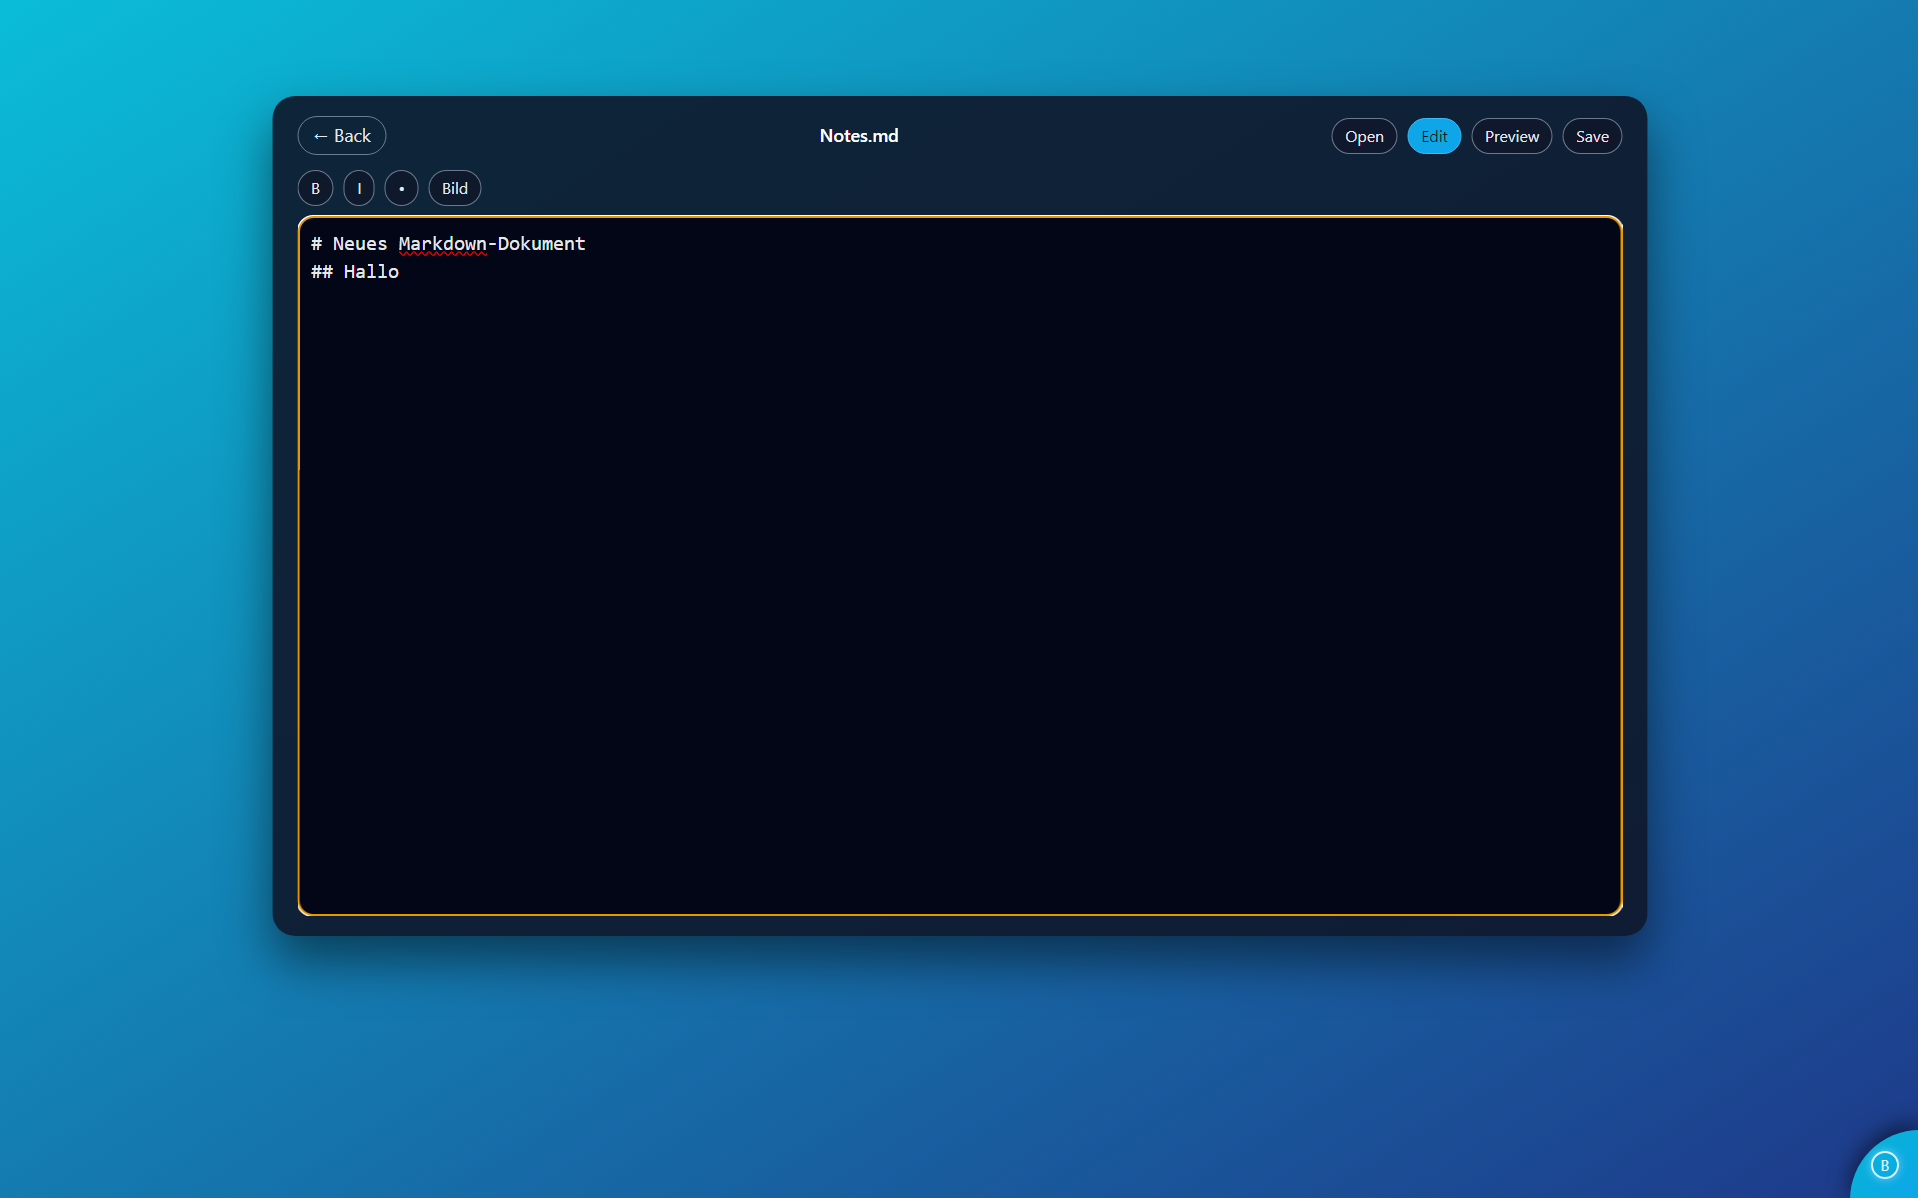
\includegraphics[width=1\textwidth]{Markdown.png}
  \caption{Markdown Editor}
  \label{fig:MD}
\end{figure}

\newpage
\subsubsection{3D- Viewer}
\paragraph{Initial implementation}\mbox{} \\
The 3D Viewer was assigned to Noah in the initial division of work and was present in the AppCarousel from at least 22 October 2025 onward. It is implemented as a React component named ThreeViewer.jsx and follows the same routing pattern as all other workbench applications, being opened and closed via the currentApp state in App.jsx.
The initial version of the viewer was deliberately minimal. It provided a basic 3D rendering environment in which a user could load and view a 3D model, but interaction was limited. Only the GLB file format was supported for import, there were no transformation tools to manipulate objects, and the scene had no grid or spatial reference to help orient the user. The camera could be orbited around the loaded model using standard mouse controls, but that was the extent of the functionality.


\paragraph{Iterative refinement}\mbox{} \\
The viewer was substantially expanded over the course of development. The final implementation relies on @react-three/fiber as the React rendering layer on top of Three.js, and makes use of the @react-three/drei helper library for higher-level controls. The full-screen Canvas component from @react-three/fiber serves as the rendering surface, configured with a perspective camera positioned at (3, 3, 3) with a 60-degree field of view.
File format support was broadened considerably. Where the first version only accepted GLB files, the final component supports four formats: GLB and GLTF files are loaded via Three.js's GLTFLoader, STL files via the STLLoader, and 3MF files via the ThreeMFLoader. Each format triggers a different loading path inside an async loadModel function. STL files, which carry only raw geometry and no material information, are automatically paired with a default grey MeshStandardMaterial so that they render correctly without requiring the user to supply any additional data. All other formats are loaded directly as Three.js scene objects. Once loaded, the model is placed at the world origin and stored both in local state and in a objectRef for later access by the export function.
A 100 by 100 unit grid was added to the scene using Three.js's built-in gridHelper, giving the user a clear spatial reference and making it much easier to judge the scale and placement of a loaded model. This addressed the disorientation that came with the original empty black void of the early version.
Transformation controls were introduced using the TransformControls component from @react-three/drei. The user can switch between three modes — Move (translate), Rotate, and Scale — using dedicated toolbar buttons. Each mode changes how the gizmo handles on the model behave, allowing full six-degrees-of-freedom positioning, free rotation around all axes, and non-uniform scaling. The active mode is stored in a mode state variable and passed down to the EditableModel child component, which wraps the loaded model inside a TransformControls instance.
A camera conflict problem was identified and addressed during development: when the user interacted with the transformation gizmo and the OrbitControls were simultaneously active, both systems competed for mouse input, causing the camera to move unexpectedly whenever the user tried to move or scale the object. The fix involved dynamically enabling and disabling OrbitControls depending on what the user is doing. When the user presses and holds the Command key (or Ctrl on Windows), orbit controls are enabled so the camera can be freely repositioned. 
\newpage
As soon as the user starts dragging a transform gizmo handle — detected via the mouseDown and mouseUp events on the TransformControls instance — orbit controls are disabled for the duration of the drag and re-enabled once the mouse is released. This gives the user reliable, conflict-free control over both camera navigation and object manipulation.
A save and export feature was implemented via Three.js's GLTFExporter. Regardless of the original import format, the current state of the model — including any transformations applied during the session — can be exported as a GLTF JSON file. The exported filename is derived from the original file's name with an edited suffix appended before the extension, so that the output is clearly identifiable. The process opens up the systems file explorer and allows the user to change the directory where the file will be stored too. 
The toolbar was styled consistently with the workbench's design language, using semi-transparent dark glass-like button surfaces with subtle border highlights and smooth hover animations driven by inline style transitions. The toolbar sits in the top-left corner of the full-screen canvas and contains buttons for: navigating back to the home screen, loading a file via a file input, switching between Move / Rotate / Scale modes, and saving the model. The scene itself is lit with a combination of ambient light and a point light, supplemented by an environment map using the city preset from @react-three/drei's Environment component, which adds physically-based ambient reflections to the model surface.

\paragraph{Performance and stability concerns}\mbox{} \\
The most significant stability issue documented during development was the control conflict between OrbitControls and TransformControls, both of which compete for the same mouse input events. In the initial implementation this caused the camera to drift or jump unexpectedly whenever the user attempted to transform an object, since both systems were active simultaneously and interpreted the same drag gesture in different ways. This was not merely a minor inconvenience but a fundamental usability problem that made precise object manipulation effectively impossible. The solution — dynamically toggling OrbitControls based on keyboard modifier state and transform gizmo interaction events — resolved the conflict, but it introduced its own complexity: the viewer now maintains two interleaved event listener systems, one on the TransformControls instance and one on the document-level keyboard events, both of which must be carefully cleaned up in their respective useEffect return functions to prevent memory leaks and stale event handlers accumulating over the component's lifetime.
From a rendering performance standpoint, the viewer uses @react-three/fiber's Canvas component which maintains a continuous WebGL render loop for as long as the component is mounted. This is appropriate for an interactive 3D editor, but it means the GPU is constantly active even when the user is not interacting with the scene. On the hardware the workbench runs on — an embedded touchscreen system rather than a dedicated workstation — this continuous rendering load is a relevant concern, particularly when other workbench applications are running concurrently in the Electron process. No frame rate cap or render-on-demand optimization was implemented, which could be a source of unnecessary resource consumption during idle periods.
Model loading is handled asynchronously inside a useEffect hook using loader.loadAsync(), and the component wraps the model in a Suspense boundary with a null fallback, meaning the UI shows nothing while a file is being parsed. 
\newpage
For small STL or GLB files this is negligible, but for large or geometrically complex models — which are common in the 3D printing context the workbench is designed for — this could result in a noticeable blank period with no loading indicator, leaving the user uncertain whether the import is progressing or has silently failed. Additionally, each time a new file is loaded a new object URL is created via URL.createObjectURL() but the corresponding URL.revokeObjectURL() call is never made, meaning the memory backing each loaded file is not released for the lifetime of the application session. In a long-running Electron session where the user loads multiple models, this constitutes a gradual memory leak.

\paragraph{Current limitations}\mbox{} \\
The 3D Viewer, while significantly more capable than its initial version, has several remaining limitations. The export format is always GLTF regardless of the input format, meaning a file originally loaded as an STL or 3MF will be re-exported as GLTF; there is no round-trip preservation of the original format. The default material applied to STL models is a flat grey and cannot be changed within the viewer, so no texturing or material editing is supported. There is no undo history, meaning any transformation applied to the model cannot be reversed without re-loading the file from scratch. The viewer also has no measurement tools or snapping functionality, which limits its usefulness for precision work beyond basic inspection and rough repositioning. Finally, although the user is able to choose the location where he wants to save the project to, he is only able to save the project in a gtlf file format. 

\begin{figure}[H]
  \centering
  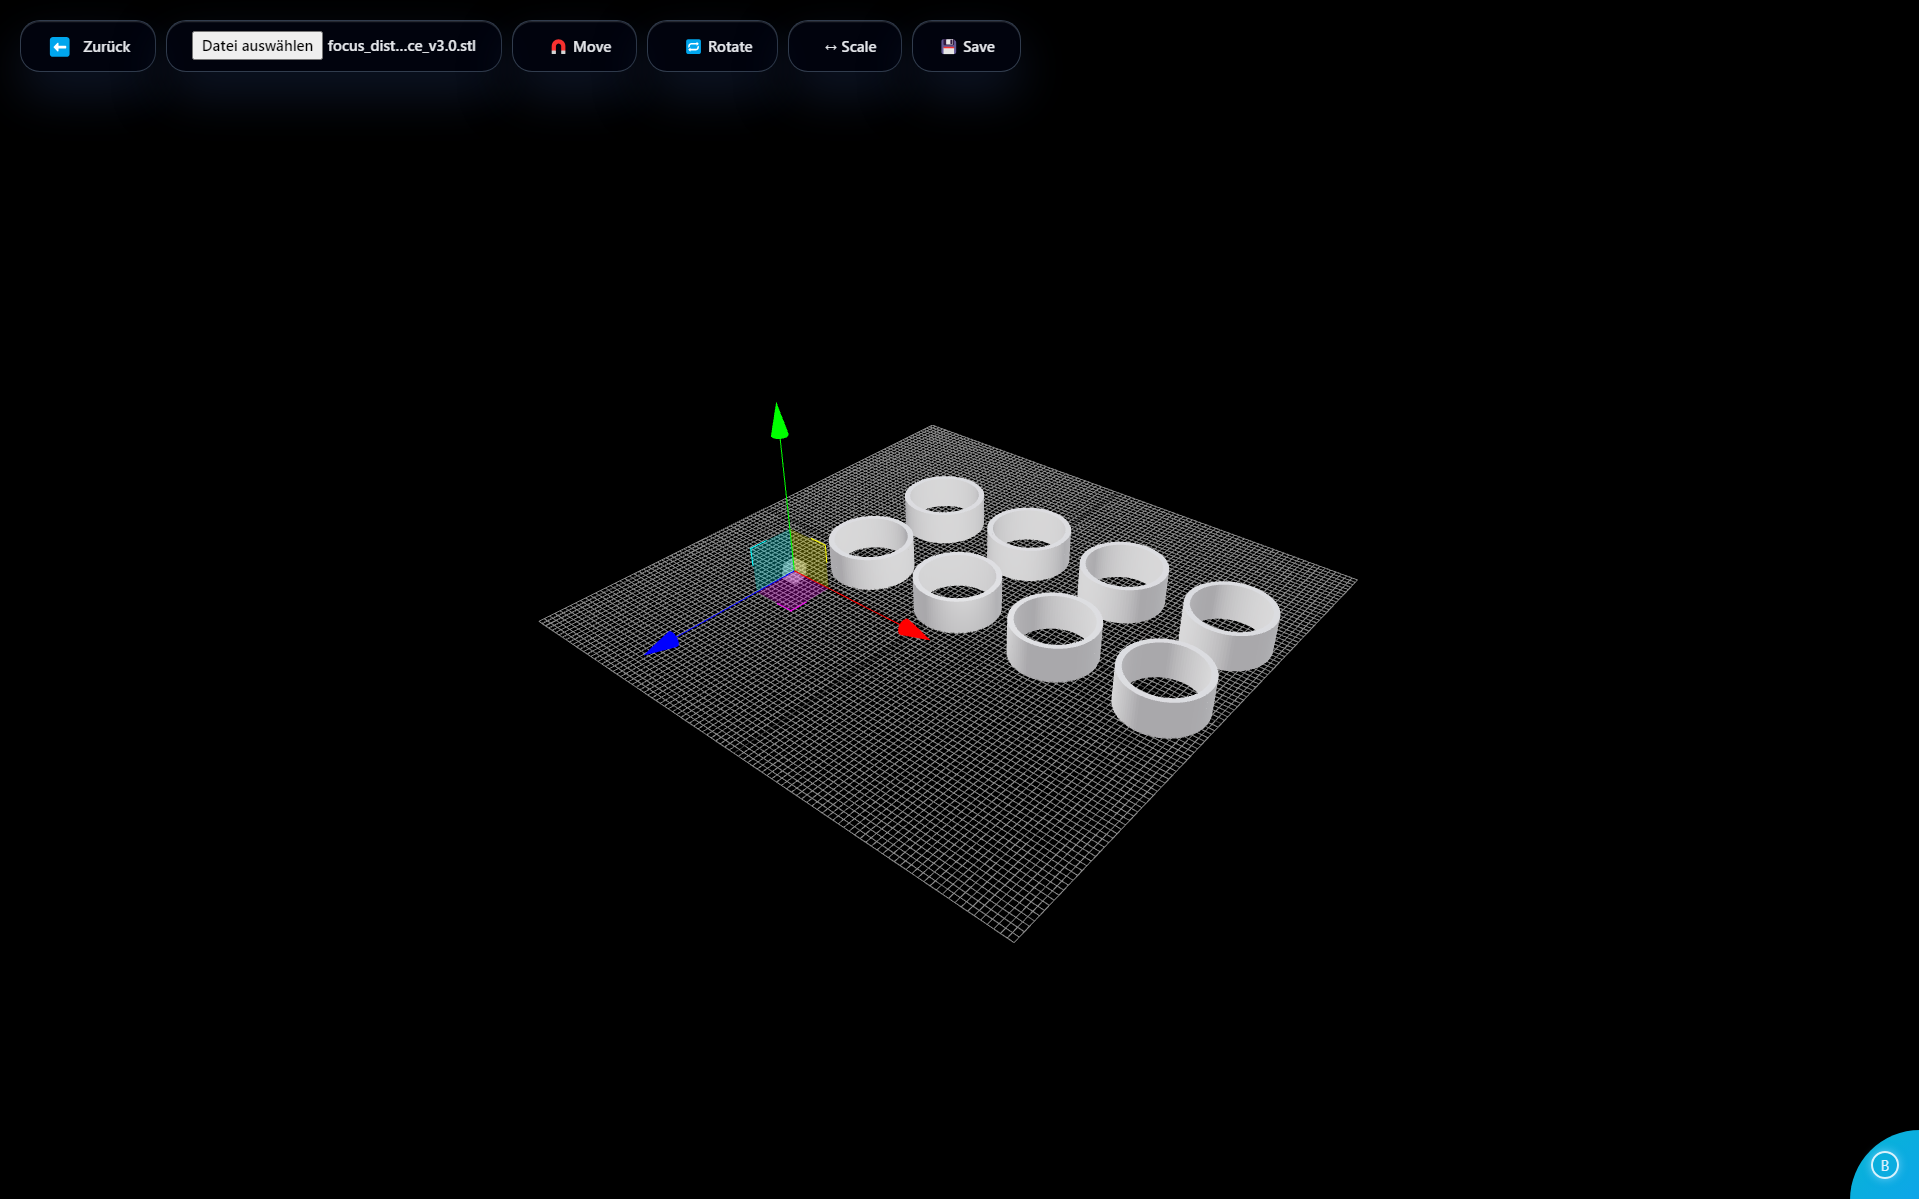
\includegraphics[width=1\textwidth]{3D_Viewer.png}
  \caption{3D- Viewer displaying an object}
  \label{fig:3D- Viewer}
\end{figure}

\subsubsection{Music library}
\paragraph{Initial Implementation}\mbox{} \\
The initial idea for the Music library got up early in development. This application got through a high amount of remodeling because of problems and discoveries while development. At the beginning of the Music library the vision was an integration of aether one of the big music streaming services such as Apple Music or Spotify.

\paragraph{Iterative refinement}\mbox{} \\
Integrating services from major streaming platforms proved to be an overly ambitious goal. The obstacles that emerged were both legal and financial in nature, and difficult to resolve within the constraints of an open-source student project without commercial backing. For Apple Music there is a need of the Apple Developer Program membership with yearly costs. Licenses and similar legal problems where to risky for this project. Licenses and similar legal problems were too risky for this project. Some of the legal problems were: No sort of function or possibility to save the music, this collided with the idea to create your own playlist on the GUI. No public or commercial usage such as restaurants and public facilities in general, you can’t guarantee this if it is an open source project, which should not bind you to any platform or rules. This problems are similar or the same on Spotify so with this the initial Installment needed a new idea.

SoundCloud was the second suggestion. It also provides a free-to-use API. For this, a request was submitted to the SoundCloud support team. After a few days, the response was not the one hoped for. The support team informed us that, due to the limited account history and visible activity of our developers on their platform, they are unable to provide the API due to security concerns related to AI requests in recent months. 

For the last and final idea for the development of the Music library, an Audio H5 player was used that provides a simple user interface and a customisable layout. The library needs to be installed for it to function. Predefined license-free tracks were also added to test the overall functionality. Data upload for MP3 files to the playlist is also supported. For these files to be added to the playlist, they must be uploaded to the designated explorer/finder folder. It is possible to upload MP3 files by dragging and dropping them or by manually copying the file into the folder. The playlist can then be controlled by the skip and back buttons in the user interface. If the end of the playlist is reached, it will begin from the first song again, creating a looping effect. In the End the decision with the Audio H5 player was made because of the clear advantages against other option In the end, the decision with the Audio H5 player was made because of the clear advantages over other options, especially considering the financial constraints of an open-source student project and the legal and privacy concerns encountered with third-party streaming services.

\newpage
\paragraph{Problems with compatible file formats}\mbox{} \\
A current and notable problem that has been identified during the development process is the fact that the supported file formats are strictly limited to the MP3 format. This means that any other form of media file or audio format will not be recognized or accepted by the Music Library. Files such as WAV, FLAC, AAC, OGG, or any other commonly used audio formats are at this point in time entirely incompatible with the system, and attempting to load such files into the Music Library will result in them being rejected or simply ignored by the application.

\paragraph{Current limitations}\mbox{} \\
The restriction to the mp3 files does not only present a problem in terms of compatibility and user convenience, but it also directly impacts and limits the overall audio quality that the Music Library is capable of delivering to the end user. Since the MP3 format is by its very nature a lossy compression format, a certain degree of audio quality is inevitably lost during the encoding process. This stands in contrast to lossless formats such as FLAC or WAV, which are able to preserve the full audio quality of the original recording without any loss of data. As a result of being locked into the MP3 format , the Music Library is therefore not capable of playing back audio at the highest possible quality, even in cases where higher quality source files may be available.
This is a limitation that should be addressed in a future version of the application in order to broaden the compatibility of the system and to allow users to enjoy a higher standard of audio playback.

\begin{figure}[H]
  \centering
  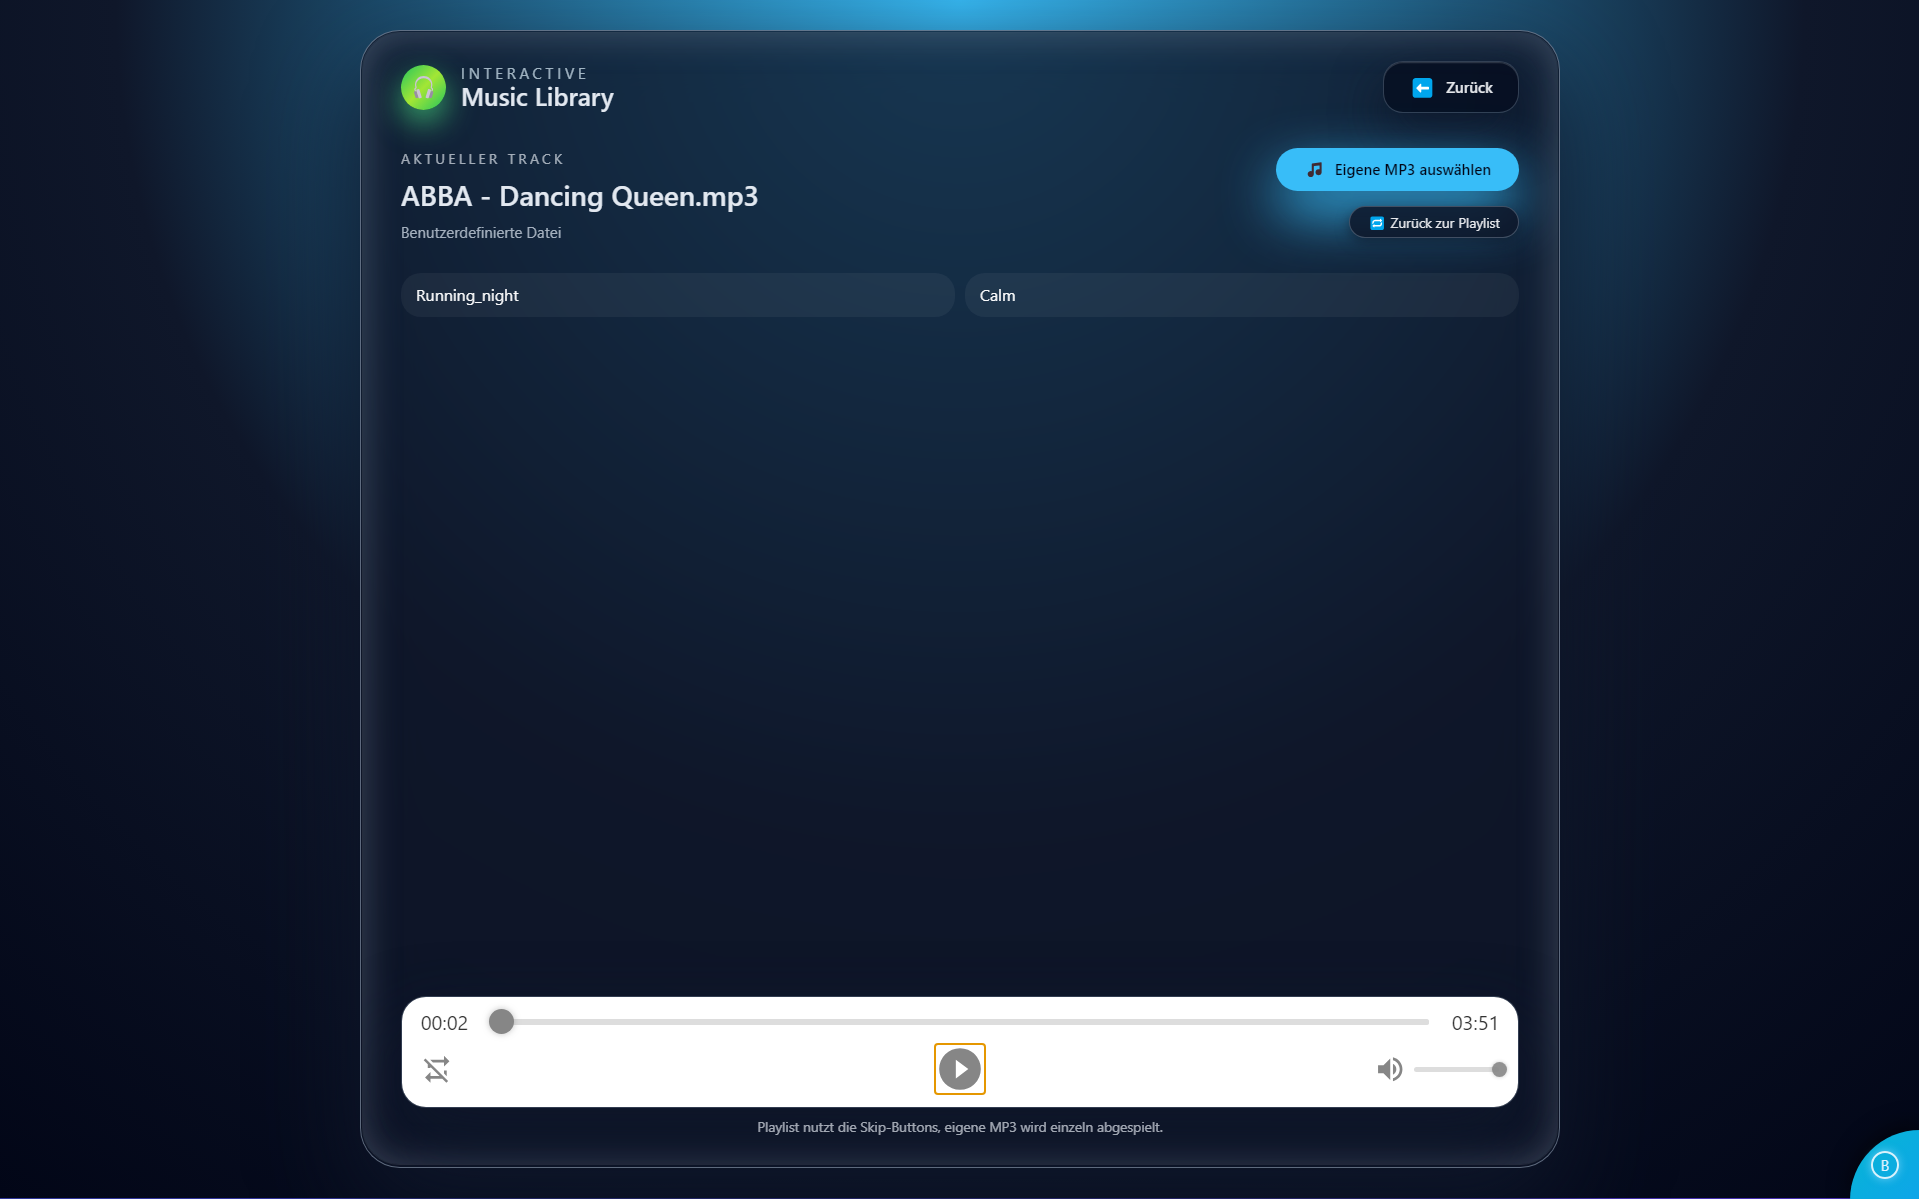
\includegraphics[width=1\textwidth]{MusicLibrary.png}
  \caption{The music library playing a song by a certain swedish band}
  \label{fig:Music}
\end{figure}

\newpage
\subsubsection{Games and casual}
\paragraph{Initial implementation}\mbox{} \\
After some time of development, focusing entirely on applications to boost the users productivity, we decided that we also want to offer the user some element of fun and joy when using the workbench. 
This led to the first idea of implementing games into the workbench, with development of the first game starting all the way back in mid- October 2025. 

The initial concept was to embed games- snake and minesweeper to be more precise- with python and context bridges to connect it to the main JavaScript application running the workbench. 
This idea was quickly pivoted towards a React-based architecture to stay consistent with the rest of the stack as well as eliminating potential compatibility and communication problems between the two different programming languages before even creating them. 

The first concrete step in this development journey was the creation of a Game Collection component, introduced on the 22 of October 2025. This component serves as a unified launcher — a library from which individual games can be selected and started. 
Each game entry in the collection is represented by a cover image (icon) suiting the game component, a title, and a short description, rendered in a responsive CSS grid layout. The first (and at that point only) entry was "Byte Invaders", a retro space shooter, identified by the ID byte-invaders. The component was integrated into the main app routing (App.jsx) and added to the AppCarousel alongside the other workbench applications.
At this stage, clicking the Byte Invaders cover image did not yet launch a game — a placeholder screen (SpaceInvaders.jsx) was implemented first, confirming that the routing and state management between GameCollection and the game screens worked correctly before any game logic was written.

\paragraph{Iterative refinement}
\subparagraph{Game collection}\mbox{} \\
The Game Collection itself went through several iterations before reaching its final form. In the first version the game cards were purely decorative — cover images and text with no interactive behaviour. In a second iteration each card's cover image was turned into a clickable button that passes the selected game's id through an onStartGame callback prop. In App.jsx, this callback sets an activeGame state variable, which then controls which game component is conditionally rendered. This introduced a clean two-level state separation: currentApp determines which top-level workbench application is open, while activeGame determines which individual game within the collection is running. This pattern proved to be robust and extensible — adding each new game required only appending one entry to the games array inside GameCollection.jsx and one additional conditional render block in App.jsx. All three games were integrated using exactly this mechanism.

\newpage
\subparagraph{Byte invaders}\mbox{} \\
Byte Invaders is a Space Invaders-style retro arcade game developed by Noah. Development began on 6 November 2025 with a functional first version, followed by a significantly enhanced second iteration on 12 November 2025.

The first version established all core gameplay mechanics. The game renders entirely on an HTML5 <canvas> element and is driven by a requestAnimationFrame-based game loop. The player controls a ship at the bottom of the screen using the arrow keys or the A/D keys, and fires projectiles upward with the spacebar. The enemy formation consists of a grid of 8 columns by 3 rows of rectangular enemies that march horizontally across the canvas. Whenever any enemy reaches the left or right boundary, the entire formation reverses direction and shifts one step downward toward the player. Player projectiles are subject to a 200ms shoot cooldown to prevent rapid-fire spam, and collision detection between bullets and enemies is handled through axis-aligned bounding-box (AABB) intersection checks.

The second version introduced a wave system, escalating difficulty, a score counter, a proper game over condition, and clean reset logic. When all enemies in a formation have been destroyed, a new full formation spawns immediately, providing continuous gameplay. The horizontal movement speed of the enemy formation increases by 0.5 units per completed wave, meaning each successive wave is perceptibly faster and more demanding. Enemy speed is stored in a useRef so that it accumulates reliably across waves without being inadvertently reset by React re-renders. The score awards 100 points per destroyed enemy and is maintained using two parallel variables: a useRef for synchronous, always-current access inside the game loop, and a useState variable for triggering UI updates. This dual ref/state approach was necessary because requestAnimationFrame callbacks close over the state value at the time of their creation, meaning a useState-only approach would produce stale score readings within the loop. A game over is triggered when any enemy reaches the player's vertical position, at which point the loop terminates and a semi-transparent overlay is rendered showing the final score and three navigation options: Restart, back to Game Collection, and back to the workbench Home screen. A dedicated resetGame() function handles a clean restart by restoring all mutable references and state variables to their initial values, including player position, bullet array, enemy formation, movement speed, and score.

\subparagraph{Snake}\mbox{} \\
The Snake game (SnakeGame.jsx) was developed by Noah and added to the workbench on 13 November 2025. It follows the classic Snake mechanics: the player steers a continuously moving snake across a bounded grid using the W/A/S/D keys or the arrow keys. Each time the snake consumes a food item, its body grows by one segment. The game ends when the snake collides with its own body or with the boundary of the play field. Like Byte Invaders, the game is rendered onto an HTML5 canvas using a requestAnimationFrame loop that updates the game state and redraws the scene on every frame. It was integrated into the Game Collection using the snake-game identifier and added to the App.jsx routing in the same way as all other games.

\newpage
\subparagraph{Minesweeper}\mbox{} \\
Minesweeper was developed by Noah concurrently with the Snake game and added to the workbench in the same time frame in mid-November 2025. Unlike the canvas-based games, Minesweeper is implemented entirely in React using standard DOM elements, meaning its state is managed directly through useState without requiring a custom render loop.

The game board is a 10 by 10 grid of cell objects, each carrying four properties: revealed, mine, flagged, and adjacent. The board is initialised empty via createEmptyBoard(), and crucially, mine placement is deferred until the player's very first click. This safe-first-click mechanic guarantees that the initially selected cell is never a mine, preventing an instant game over on the opening move. Once the first cell is clicked, 15 mines are distributed randomly across the remaining cells. After placement, the adjacency counter of every non-mine cell is computed by checking all eight of its neighbours and counting how many contain a mine.

Left-clicking a cell triggers handleCellClick(), which creates an immutable copy of the board, optionally plants mines on the first interaction, and then calls the recursive reveal() function. If the clicked cell is a mine, it is revealed with a red background and the game ends immediately. If the cell has a non-zero adjacency count, only that single cell is uncovered and its number is shown. If the adjacency count is zero — meaning no neighbouring mines — the reveal function propagates recursively in all eight directions, flood-filling outward and uncovering all connected zero-cells and their numbered borders in a single action. This flood-fill is what allows large safe areas to open up with one tap. After each reveal, a win condition is evaluated: if every non-mine cell on the board has been uncovered, the player wins.

Right-clicking an unrevealed cell toggles its flagged state. Flagged cells display a icon and are protected from being accidentally revealed by both direct clicks and the recursive flood-fill. The board is rendered as a CSS grid of 32 by 32 pixel cells. Unrevealed cells appear in dark grey, revealed safe cells in light grey, and detonated mine cells in red. Adjacency numbers follow the classic Minesweeper colour convention: 1 in blue, 2 in green, and values above 2 in red. When the game concludes — either through a mine detonation or a fully cleared board — a semi-transparent overlay presents the result and offers the same three navigation options as the other games: Restart, Game Collection, and Home.

\subparagraph{Solar system simulation}\mbox{} \\
The Solar System simulation (SolarSystem.jsx) was developed by Alex and introduced on 12 November 2025, with moons and final textures added the following day. It uses the Three.js library to render a real-time, interactive 3D model of the solar system inside the Electron-based workbench environment.

All planets are represented as Three.js mesh objects with spherical geometry, orbiting a central sun. Each planet follows a circular orbital path with its own angular velocity, set to visually plausible relative values rather than astronomically precise ones, keeping the simulation readable and engaging on screen. When the user selects a planet, the camera transitions smoothly and locks onto that body while an information box appears displaying contextual data about it. 

\newpage
This camera focus animation interpolates the camera's position and target across several frames to produce a fluid transition rather than a hard cut.
In the second iteration moons were added to the relevant planets, each following its own orbital path around its parent body. Planet and moon textures were sourced as image assets and stored in the project's public folder, then applied as Three.js texture maps to the respective mesh materials. 

Unlike the games in the Game Collection, the Solar System is registered as a standalone entry in the AppCarousel array under the name "Solar System", placing it at the same level as other workbench applications such as the Paint tool, the File Manager, and the Weather app.

\subparagraph{Touch input capability}\mbox{} \\
All games were initially built with keyboard input only, which was insufficient for the workbench's intended use on a touchscreen monitor. Touch compatibility was addressed as a dedicated effort on 22 January 2026.
For Snake, touch input was added via onTouchStart and onTouchEnd event handlers attached directly to the canvas element. A touchStartRef captures the coordinates of the initial touch point. When the finger is lifted, the displacement vector (dx, dy) is computed and compared against a TOUCH-THRESHOLD of 40 pixels; displacements below this value are treated as accidental taps and discarded. Valid swipes are passed to a handleSwipeDirection() function that maps the dominant axis and direction of the vector to one of the four movement directions.

Byte Invaders required a different approach because it relies on continuous directional input — the player must hold a key to keep moving — rather than discrete swipe events. A persistent on-screen control bar was therefore added below the game canvas containing three touch buttons: move left (<-), move right (->), and shoot. Each button updates a touchInput ref object on onTouchStart (activate) and onTouchEnd (deactivate). Inside the game loop, keyboard and touch inputs are merged so that either input source can drive the player: for example, isShooting = keys.current.shoot || touchInput.current.shooting. An e.preventDefault() call on every touch handler prevents the application from interpreting game interactions as page-level scroll or zoom gestures, which would otherwise conflict with the canvas.

Minesweeper required no dedicated touch work. Because it is built from standard DOM elements driven by click and context-menu events, the apps default behaviour of mapping touch taps to click events was sufficient for full touch compatibility without any additional code.
\newpage
\paragraph{Stability and performance concerns}\mbox{} \\
The main stability concern documented during development relates to the lifecycle management of requestAnimationFrame game loops inside React components. When a game component unmounts — for instance when the player navigates back to the Game Collection — the active animation loop must be explicitly canceled to prevent it from continuing to run in the background and accessing stale or deallocated references. In the initial implementation of Byte Invaders, cancellation was handled only by an isGameOver guard at the top of each loop iteration rather than by a proper cancelAnimationFrame call. 

The diary acknowledges that the correct solution is to store the most recent animation frame ID in a ref and cancel it from within the useEffect cleanup function, though this was not yet fully applied at the time of writing.
A second concern arose from React's asynchronous state update model. Score values maintained exclusively through useState produced stale reads inside the synchronous game loop, causing incorrect score displays. This was resolved by the dual ref/state pattern described above, which became a recurring design convention across the game implementations.
For the Solar System, the use of Three.js for continuous 3D rendering via WebGL introduces a higher baseline CPU and GPU load compared to the 2D canvas-based games. 

No specific performance issues were recorded in the diary, but this is an inherent characteristic of real-time 3D rendering in an Electron-hosted application context.

\newpage
\paragraph{Current limitations}\mbox{} \\
Several limitations were apparent across the game and simulation implementations at the time documented in the diary. Byte Invaders has no enemy projectiles, meaning difficulty scales solely through movement speed rather than through increased threat complexity. None of the games implement persistent score storage; all scores are held in React state and are lost when the component unmounts, with no high-score mechanism via local storage or a backend. The Game Collection's game registry is hard-coded as a static array inside GameCollection.jsx, so every new game requires a manual update to both this array and the routing logic in App.jsx — there is no dynamic registration mechanism. Touch controls are not uniform across games: Snake uses swipe gestures while Byte Invaders uses on-screen buttons, which may produce an inconsistent experience for users. The Minesweeper board dimensions and mine count are fixed constants with no difficulty settings exposed to the player. Finally, the Solar System simulation is a visual demonstration rather than a physically accurate model — orbital periods, distances, and sizes are approximated for visual clarity, and no gravitational mechanics are simulated beyond the predefined circular orbits.

\begin{figure}[H]
  \centering
  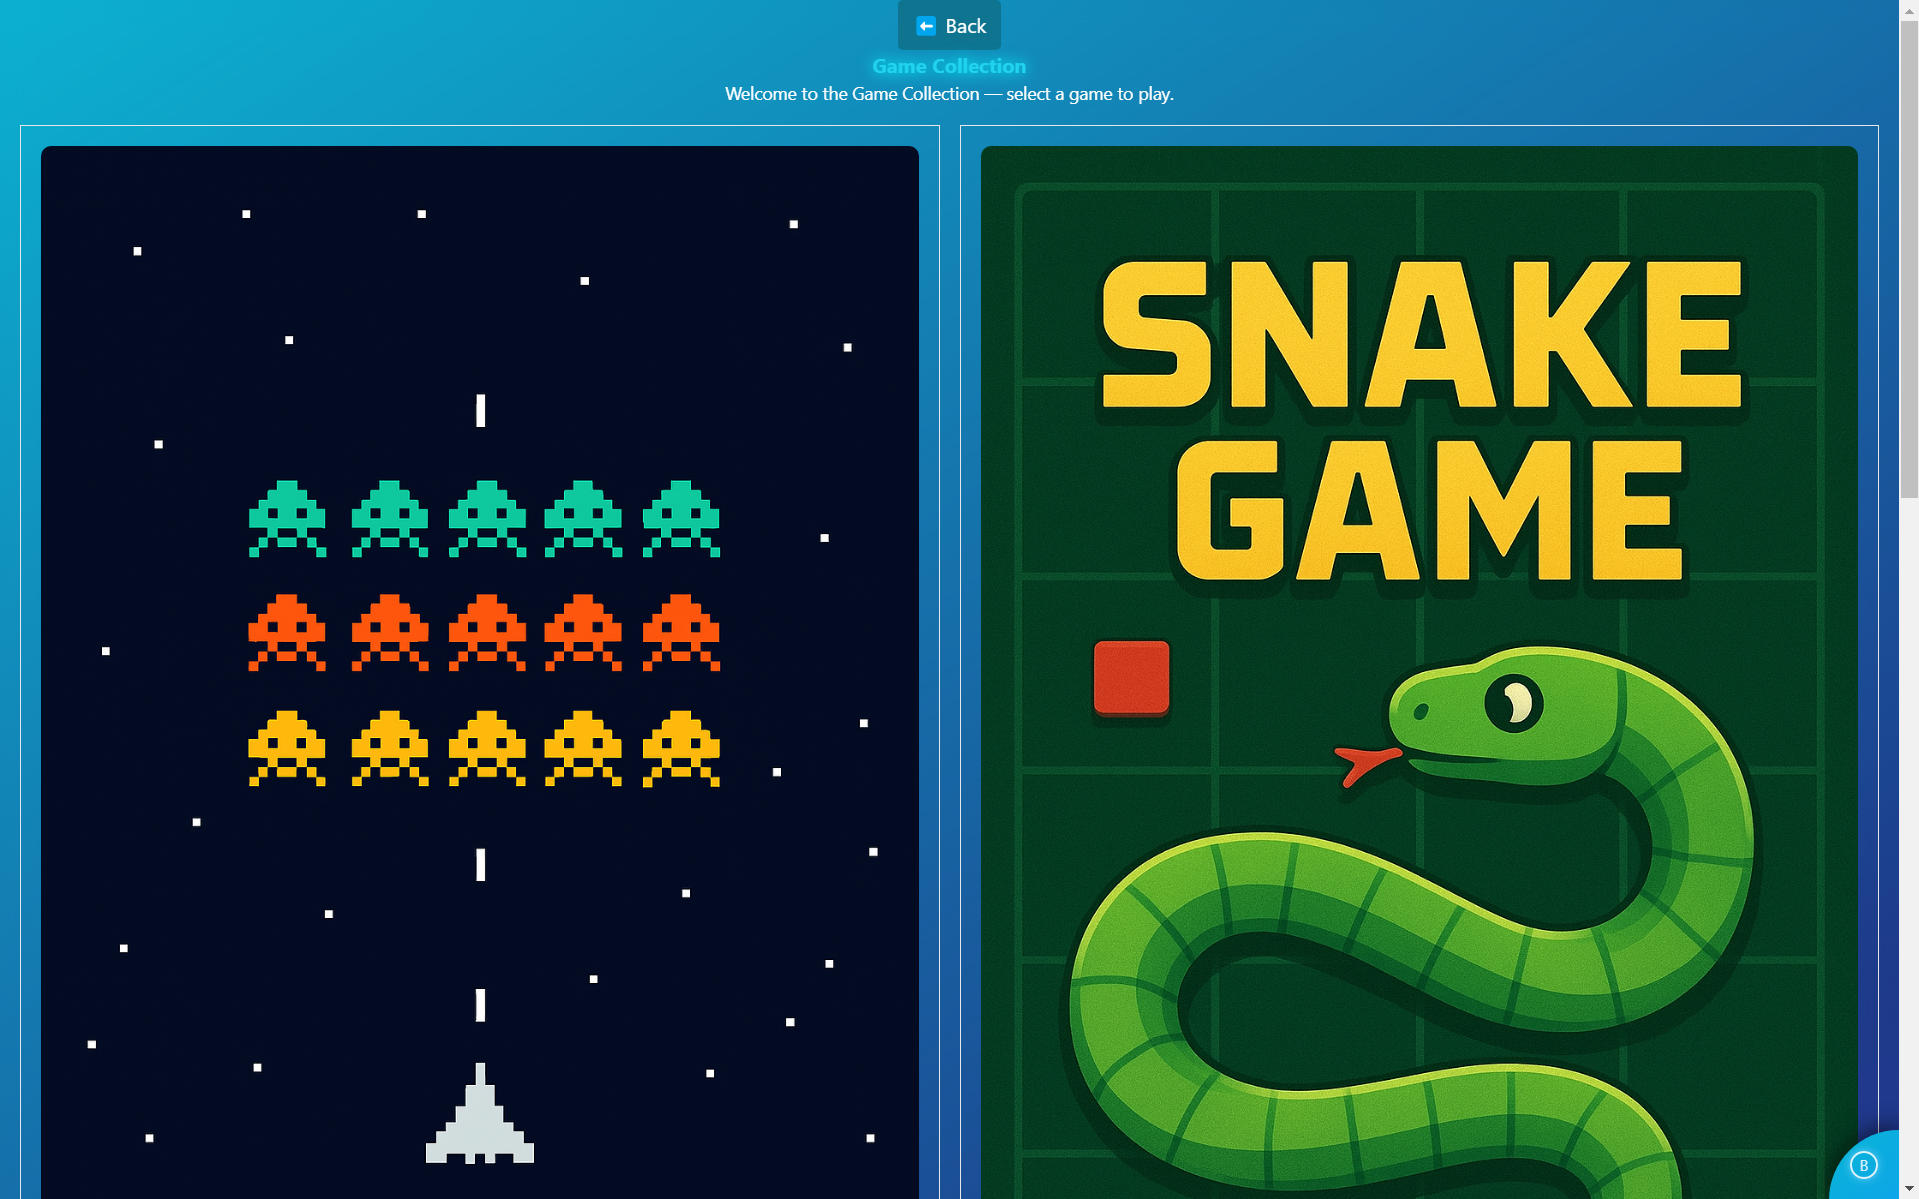
\includegraphics[width=1\textwidth]{GameCollection.png}
  \caption{The GameCollection}
  \label{fig:Games}
\end{figure}

\newpage
\subsubsection{Expandability through app integrations}
\paragraph{Open source application integrations} 
\subparagraph{Motivation and Approach} \mbox{} \\
A core goal of the workbench was to serve as a practical tool for a 3D printing and engineering context. This meant that professional-grade software for slicing 3D models and designing parts needed to be accessible from within the workbench interface. The team initially considered building a slicer from scratch, but after research concluded that a functional slicer requires a team of 20 or more experienced developers and is far outside the scope of a two-person diploma project. The decision was therefore made to integrate existing open-source applications — OrcaSlicer, FreeCAD, and later Bambu Studio — directly into the workbench rather than attempting to replicate their functionality.
This approach came with an acknowledged trade-off: none of these external applications match the workbench's visual design language. They open in their own native windows with their own UI, breaking the immersive, themed aesthetic of the rest of the platform. The team were candid in the diary about not being entirely happy with this compromise, but accepted it as the only realistic path to providing this category of functionality.
The integration pattern used for all three applications is identical in structure. Each is represented by a React component in the workbench's frontend that auto-launches the external program when opened, communicates with Electron's main process via the electronAPI IPC bridge exposed through preload.js, and is added to the AppCarousel so it appears alongside the natively built workbench tools.

\subparagraph{OrcaSlicer}\mbox{} \\
OrcaSlicer — more specifically the Orca for Flashforge variant — was the first external application to be integrated, implemented by Noah on 16 October 2025. It was also the first application in the entire project that does not live inside the workbench's React frontend but instead runs as a completely separate native process.
The frontend component, OrcaSlicer.jsx, is minimal by design. When it mounts, a useEffect hook immediately calls window.electronAPI.launchOrcaSlicer(), which sends a launch-orca-slicer IPC message to Electron's main process. The main process handles this message by resolving the hard-coded path to the OrcaSlicer executable, spawning it as a detached child process with stdio set to ignore, and then calling child.unref() to allow the slicer to continue running independently even if the workbench process itself were to close. The workbench-side screen shown to the user while the slicer is launching is a simple placeholder that confirms the launch is in progress, with a Back button to return to the home screen. There are no controls, no file interaction, and no communication between the workbench and the slicer once the process has been spawned — the user works with OrcaSlicer in its own window entirely outside the workbench's control.
\newpage
\subparagraph{FreeCAD}\mbox{} \\
FreeCAD was assigned to Alex and follows the same launch-and-forget integration pattern as OrcaSlicer. When the FreeCAD entry is selected from the carousel, the corresponding component triggers the openfreecad IPC command, which in main.js spawns the FreeCAD executable as a detached, independent process. FreeCAD then opens in its own native window and the workbench effectively hands off to it entirely.
The FreeCAD integration was one of the first places in the project where cross-platform path handling was explicitly addressed. The main process checks process.platform to determine the operating system: on Windows it resolves the path to freecad.exe inside the user's local application data directory, while on macOS it uses the exec('open -a /Applications/FreeCAD.app') command to launch the application bundle through the system's standard open mechanism. This platform branching became a template that was reused across subsequent integrations.

\subparagraph{Bambu Studio} \mbox{} \\
Bambu Studio was added on 18 December 2025 as a third slicer integration, targeting Bambu Lab's own 3D printing ecosystem. The implementation follows the same structure as OrcaSlicer and FreeCAD but was notable for introducing a concrete bug during development. The initial version of BambuStudio.jsx called 

window.electronAPI.launchBambuStudio() directly inside an if condition that was checking for the function's existence. Because calling a function returns its return value — in this case undefined — the condition always evaluated to false, meaning the slicer never actually launched and the "Electron bridge not available" error alert was displayed every time even though the bridge was working correctly. The fix was straightforward: check for the function's existence first, and then call it separately inside the block if it is present. Like the other integrations, the spawned process is detached and unreferenced so it runs independently of the workbench.

\subparagraph{Stability improvements and the safeSpawn pattern} \mbox{} \\
On 7 January 2026, a broader stability pass was made specifically targeting all external application launches. The diary notes that a more failsafe main.js platform query was introduced and applied uniformly to every non-natively developed application — BambuStudio, FreeCAD, and OrcaSlicer — rather than having each integration handle its own error cases inconsistently. This consolidation reduced code duplication and made the launch behaviour more predictable across the three integrations. A safeSpawn helper was also introduced as a wrapper around the raw Node.js childprocess.spawn call, providing centralised error handling for cases such as a missing executable, an incorrect path, or a system-level permission error. Rather than crashing the Electron main process or silently failing, safeSpawn catches these errors and logs them clearly, making the source of a failed launch much easier to diagnose.

\newpage
\subparagraph{AI-Triggered launching} \mbox{} \\
Beyond being accessible as tiles in the app carousel, all three external applications were later wired into the workbench's AI assistant as part of a broader effort to make the platform feel more interactive and voice-driven. On 21 January 2026, the Python ChatAssistant.py backend was extended with a Command data model and a keyword scanning step that runs on every incoming user prompt. If the text contains trigger phrases such as "freecad", "starte freecad", "bambu studio", or "starte bambustudio", the assistant constructs a Command object identifying the target application and returns it alongside the normal language model reply. The frontend then forwards this command to main.js via the executeCommand IPC bridge. Before executing, the main process shows the user a native confirmation dialog — "Assistant wants to run: openfreecad. Continue?" — requiring an explicit Allow before spawning the process. This consent step was a deliberate design decision to prevent the AI from silently launching applications without the user's awareness. By the end of January 2026, this voice-triggered launch mechanism was confirmed working for OrcaSlicer, FreeCAD, and Bambu Studio.

\begin{figure}[H]
  \centering
  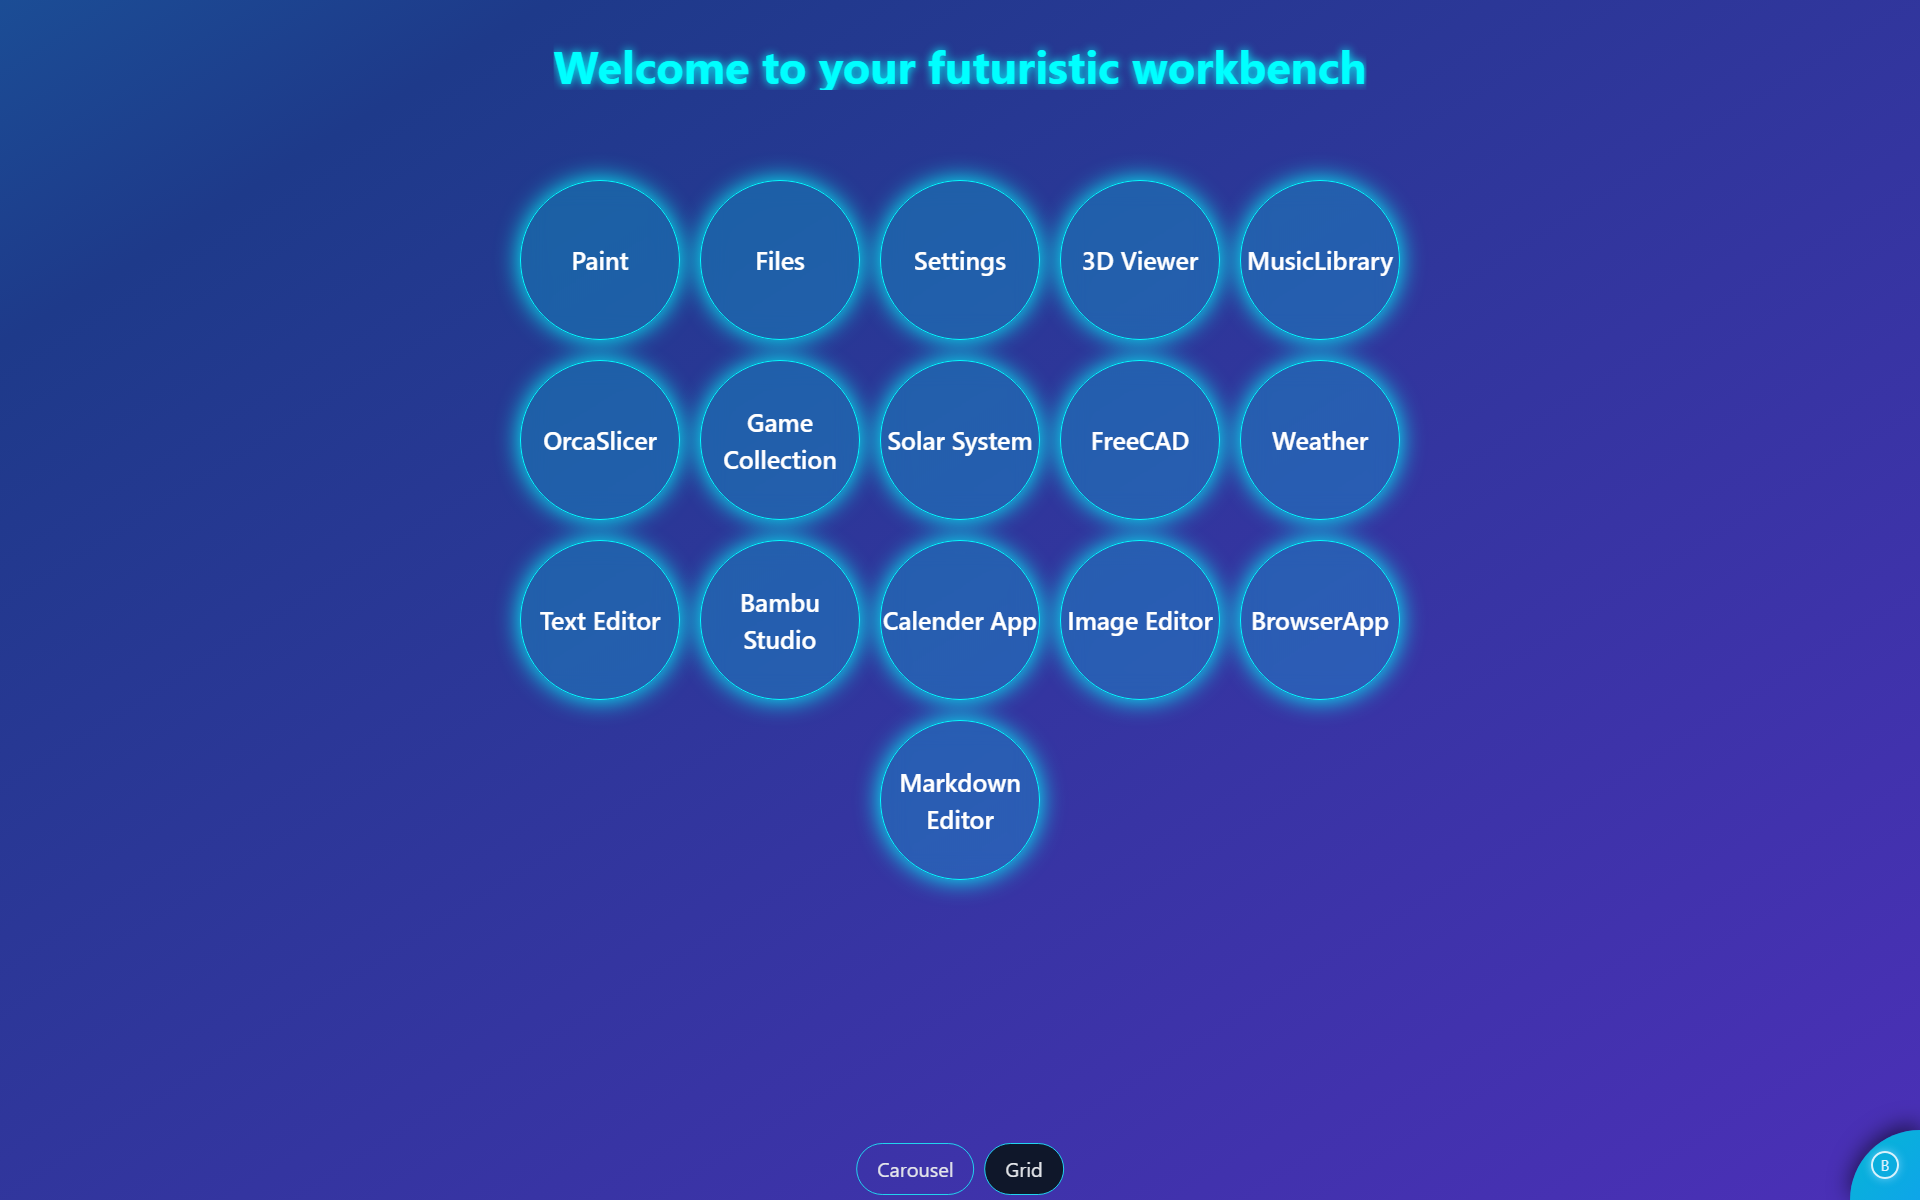
\includegraphics[width=1\textwidth]{Screenshot (34).png}
  \caption{Overview of all applications}
  \label{fig:View}
\end{figure}

\newpage
\subsection{Frontend software development}
The Design of the workbench is a essential and crucial choice. One of the main points for the workbench is a simple and modern looking GUI, that was something to always consider during the development process, yet it should be optimized for efficiency and compatible with older hardware. 

In the beginning of development, the first prototype design was made with the use of React. This prototypes design was focused on functionality and structure, rather then visual refinements. For this, basic className assignments were used. With that, it was possible to have a rapid and yet functional development process. 

After further development it became important to have a overall design and functionality for the whole GUI. The choice fell on CSS (Cascading Style Sheets), because as a Stylesheet-language it could be added without difficulty to our JavaScript based code. CSS made a clear separation between structure and design, improving the readability of the code and the process of generalization of the design over all applications. 

For the general design we chose a transparent look with blue accents, which makes our GUI look on time with the overall design of modern GUIs. Buttons got interactive designs in our GUI such as subtle hover effects, when your mouse is over a distinct button. In the settings application, the user can select from several color schemes that apply to the background and application icons. The themes do not currently extend to the interior of individual applications. It was made sure that even with the transparent look a good readability and contrast were guaranteed. The design is also equipped with a satisfactory amount of icons to simplify the recognizing of distinct buttons and make the navigation more beginner friendly.

\newpage
\subsubsection{Evolution of animations}
The first development of a animation within the project was implemented in the context of the boot-up sequence of the Workbench. Alex implemented this in the form of a smooth and slow zoom-in animation, in which the logo of the Workbench gradually appears on the screen and slowly expands in size, giving the startup screen a polished and professional feel. Alongside this, the text "Welcome to Holomat!" is displayed using a Typewriter Effect, meaning that the individual characters of the text write themselves out one by one in the center of the bottom half of the screen, rather than appearing all at once. This combination of the zoom-in logo animation and the Typewriter Effect gives the boot-up screen a dynamic and visually engaging appearance, making it a fitting introduction to the application.

The development of the animations and the overall design language of the project also brought a number of different challenges and problems that had to be tackled along the way. One of the first and most notable of these challenges arose from an idea that Alex had for the background of the Workbench. The original concept was to implement an animated background in the style of the classic Apple Mac screensavers, in which a variety of colorful strings would appear to be "flying" through space, creating a lively and visually dynamic environment for the user interface.

An initial prototype of this concept was built using HTML and showed a considerable amount of potential at first glance. The animation looked visually professional and gave the Workbench a distinctive and engaging atmosphere. However, despite its appealing appearance, the problems that came with it quickly proved to be too overwhelming to ignore. The performance of the animation told a completely different story compared to its visual quality. Even when running on proper and capable development hardware, the machine began to heat up noticeably fast, making it very clear that the animation was placing a significant load on the system. These signs made it obvious that the animation would require a substantial amount of optimization before it could properly fulfill its intended purpose within the application.

Because of these performance concerns, the decision was made to move away from the original concept entirely and to go back to a simpler but equally effective alternative. The new approach for the background animation was based on the idea of a subtle and continuously looping color transition, shifting between a blue and a darker shade of blue. This transition flows in a directional loop, starting from the bottom right corner of the screen and gradually moving towards the top left corner, creating a smooth and gentle movement across the entire background. While this solution is considerably more understated compared to the original flying strings concept, it achieves a similar goal of giving the Workbench a living and breathing feel without placing any significant load on the system. The result is a clean and visually appealing background animation that complements the overall design language of the application while remaining fully optimized for performance.

\newpage
\subsubsection{Evolution of the design}
The overall design of the Workbench had to go through a longer and more involved development process, which is not uncommon in the context of a graphical user interface, where the visual design plays an especially important and defining role for the quality and feel of the entire program. What the user sees and interacts with on a daily basis is shaped heavily by the design decisions made during development, which is why this aspect of the project required a considerable amount of iteration and refinement over time.

The very first designs that were created for the prototypes of the different applications, buttons, and controls were at most simple and plain inline styles, styled with a basic blue color and lacking any form of transparency or visual depth. While these early designs were sufficient for the purposes of initial prototyping and functionality testing, they were far from the polished and cohesive visual identity that the Workbench would eventually take on. It was through the continued development and refinement of the interface that transparency became one of the most defining and important elements of the overall design language, ultimately shaping the final appearance of the Workbench in a significant way.

After the first implementations of the design had been completed, a few weeks into the development process Alex came to the insight that the overall design language of the Workbench needed to be fundamentally reworked and finalized in its appearance. The goal was to establish a clear and consistent visual rulebook that all future applications within the Workbench could refer back to, ensuring that the entire graphical user interface would feel cohesive, unified, and intuitive for the end user.

As previously mentioned, transparency had already emerged as an important factor in the design vision. The core idea from Alex was that the design should be timeless, modern, and performance efficient all at once, striking a balance between visual appeal and technical practicality. In the pursuit of these goals, it became clear that CSS was a far more organized, maintainable, and reliable approach to styling compared to the use of inline styles, which had served their purpose during the early prototyping phase but were no longer suitable for a fully developed and scalable user interface.

With this new direction in mind, the entire graphical user interface was redesigned from the ground up. The new design language featured transparent buttons with a subtle blue shine, giving the interface a sleek and modern appearance. A gentle increase in size was added as a hover effect, providing the user with clear and satisfying visual feedback when moving the mouse over buttons and interactive elements. The overall applications were styled in a blue and cyan color scheme, tying the entire Workbench together into a consistent and polished visual identity.
The design had to be redone several times- why? How? Problems like the design changes not working etc could be covered here and there fix could be covered here. 

\newpage
\section{Discussion}
The final implementation of the Interactive Workbench fulfills the core objectives defined at the outset of the project, delivering a modular, touch-optimized digital environment that consolidates a broad range of practical tools within a single unified interface. The platform covers domains ranging from 3D manufacturing and software development to AI-assisted interaction and casual entertainment, demonstrating both the versatility of the chosen architecture and the feasibility of the underlying concept.

The development process was not without significant challenges. Throughout the project, time proved to be one of the most constrained resources. Technical difficulties — particularly those arising from cross-environment integration and touch input compatibility — frequently required unplanned debugging effort, which reduced the time available for feature development. A recurring pattern emerged in which the introduction of a new feature would expose previously hidden issues elsewhere in the system, making sustained progress difficult at certain stages of development. Despite this, every challenge encountered was ultimately resolved, and no issue proved permanently blocking to the project's completion.

Workload distribution and team coordination, managed through GitHub's project and repository tooling, played an important role in maintaining progress throughout the development period. The structured division of responsibilities ensured that there was always active development taking place across different components of the system, which helped sustain momentum even during more demanding phases of the project. That said, coordinating a project of this complexity as a two-person team introduced its own difficulties, and periods of reduced availability due to attendance and health-related absences required additional effort to recover through overtime work outside of scheduled development time.

Nevertheless we pursued through all the trouble and inconsistencies in motivation and performance. 
\newpage
\subsection{Development issues}
Several technical challenges emerged during development that had a measurable impact on both workflow efficiency and overall time management.

A recurring difficulty involved the frontend styling approach. Rather than establishing a consistent and structured CSS strategy from the beginning, styling decisions were made incrementally as development progressed. This led to inconsistencies across components and required significant refactoring effort later in the project, as design rules that should have been centralized were instead scattered across individual files. A more systematic approach to styling architecture from the outset would have reduced this overhead considerably.

The integration of the AI assistant presented another major technical challenge. The implementation required stable communication between the JavaScript-based frontend and a Python-based backend process, a cross-environment dependency that introduced recurring issues including connection errors, execution inconsistencies, and timeout-related server crashes. Resolving these problems demanded substantial debugging effort and careful architectural restructuring before reliable inter-process communication could be achieved.

Perhaps the most pervasive challenge throughout the project was the requirement to make every component of the workbench compatible with touch input. This constraint influenced design decisions across all applications and frequently required unconventional solutions. The Byte Invaders game serves as a clear example: standard swipe-based directional input was insufficient for continuous movement control, necessitating the development of persistent on-screen touch buttons as an alternative interaction model. Ensuring consistent and intuitive touch behavior across applications with fundamentally different interaction requirements proved to be one of the most time-consuming aspects of the project.

Portability and cross-platform compatibility introduced additional complexity throughout development. Ensuring stable and consistent behavior across Windows, macOS, and Linux required careful attention to platform-specific differences in path handling, process spawning, and rendering behavior, as discussed in detail in the Technical Specifications chapter.

Version control and project management through GitHub, while essential to the development process, also presented difficulties. As the project grew in scope, the team maintained both a repository and a project board. Insufficient attention to branch management in the early phases led to long-lived development branches that diverged significantly over time, resulting in complex and occasionally problematic manual merge operations. These issues reflect a maturation in the team's approach to collaborative development that occurred progressively throughout the project.
\newpage
\subsection{Review of the project realization}
Reflecting on the development process as a whole, a number of the challenges encountered can be attributed to limited prior experience with the chosen technology stack. The learning curve associated with JavaScript, React, CSS, and Electron's cross-process communication model contributed to inefficiencies during the earlier phases of the project, where architectural decisions were sometimes made without a full understanding of their downstream consequences. In hindsight, a more thorough evaluation of these decisions — particularly regarding frontend structure, CSS architecture, and AI integration — during the planning phase would have reduced the amount of refactoring required later.

The GitHub workflow issues similarly reflect this maturation process. As the project grew in complexity, the team's approach to branch management and merging strategy evolved considerably, though not always without friction. The difficulties encountered with long-lived branches and manual merges were ultimately a consequence of both limited experience with collaborative version control at this scale and an initial underestimation of the discipline required to manage a project of this scope effectively through GitHub.

Despite these setbacks, the iterative development methodology proved to be well-suited to the project's needs. The ability to implement, evaluate, and refine components in successive cycles allowed the team to recover from technical obstacles without compromising the overall direction of the project. The workbench as delivered meets the functional and architectural requirements defined at the outset, and the development process as a whole represents a substantial gain in practical engineering experience across system architecture, cross-platform development, and project management.
Nevertheless, the iterative development approach allowed continuous refinement of the system. Despite setbacks, the project objectives were achieved, and the final workbench fulfills the defined functional and architectural requirements. The development process therefore represents not only a technical achievement but also a substantial learning experience in project planning and system design.

\newpage
\subsection{Recommendations for further improvements}
The current implementation of the workbench provides a solid and extensible foundation, and several directions for future development have been identified based on the experience gained during this project.

The theming system currently applies selected color schemes only to the application icons and home screen background. Extending theme support to the interior of individual applications would produce a significantly more cohesive visual experience and bring the design language into full consistency across the platform.

The AI assistant, while functional, remains constrained by the performance limitations inherent to running a large language model locally on consumer hardware. A more capable and responsive AI integration would substantially improve the usability and perceived modernity of the platform. Future development in this area should preserve the local-first processing approach to maintain the data security guarantees established in the current implementation. It is worth noting that an improved version of the AI assistant is already in private development at the time of writing.

General system performance represents another area for improvement. On mid-tier hardware the workbench operates satisfactorily, but noticeably slower than on 
higher-specification machines. 
Performance differences between operating systems — particularly between Windows and macOS — were also observed during development. Future versions of React and npm may address some of these differences, and targeted rewrites of performance-critical components could further improve responsiveness across hardware configurations.

The hard-coded executable paths used to launch external applications such as OrcaSlicer, FreeCAD, and Bambu Studio represent one of the most significant practical limitations of the current implementation. Any device that installs these applications to a non-standard directory will encounter launch failures. This could be addressed by implementing an automatic path detection mechanism or providing a user-configurable path settings interface.

The game collection's current architecture requires manual changes to both the application routing logic and the collection registry whenever a new game is added. As the collection grows, this approach becomes increasingly fragile. A self-registering plugin system — in which each game declares its own metadata and the collection assembles itself dynamically at runtime — would be considerably more maintainable and scalable. Related to this, persistent score storage is entirely absent from the current game implementations. Given that the workbench already runs within Electron and has access to the local filesystem, implementing high-score persistence via a local JSON file would be straightforward and would meaningfully improve the replay value of the game collection.

\newpage
The 3D Viewer's export functionality is currently limited to the GLTF format regardless of the original input format. Since STL is the dominant format in the 3D printing workflow the workbench is designed to support, users who import STL files and wish to re-export them after applying transformations are forced to convert the output before it can be used in a slicer. Supporting STL as an export format — or preserving the original input format where possible — would make the viewer a considerably more practical component of the 3D printing workflow.

Finally, the integrations with OrcaSlicer, FreeCAD, and Bambu Studio are currently unidirectional — the workbench can launch these applications but has no awareness of what occurs within them. Deeper bidirectional integration, such as monitoring a known output directory for newly exported files and surfacing them as shortcuts within the 3D Viewer, or reading slicer log output to surface status information within the workbench interface, would strengthen the platform's identity as a genuine unified hub rather than simply a launcher for external tools.

\newpage
\section{Directories}
\subsection{List of illustrations}    

\listoffigures

\subsection{About style and form}
As you may have noticed this diploma thesis leans heavy towards the technical documentation of our project while trying to keep a simplistic style and form which are meant to help the user understand this thesis better. 
This is achieved through technical explanations kept simple and short at most, helping to boost readability and understandibility. 

\newpage
\section{Bibliography}

\begin{thebibliography}{99}

% Frameworks and Runtime Environments
\bibitem{react}
Meta Open Source.
\textit{React -- A JavaScript Library for Building User Interfaces}, 2013.
Available at: \url{https://react.dev}

\bibitem{nodejs}
OpenJS Foundation.
\textit{Node.js -- Asynchronous Event-Driven JavaScript Runtime}.
Available at: \url{https://nodejs.org/docs/latest/api/}

\bibitem{electron}
OpenJS Foundation.
\textit{Electron -- Build Cross-Platform Desktop Apps with JavaScript, HTML, and CSS}.
Available at: \url{https://www.electronjs.org/docs/latest}

\bibitem{vite}
\textit{Vite -- Next Generation Frontend Tooling}.
Available at: \url{https://vitejs.dev}

% 3D Rendering and Visualization
\bibitem{threejs}
\textit{Three.js -- JavaScript 3D Library}.
Available at: \url{https://threejs.org}

\bibitem{r3f}
Pmndrs Collective.
\textit{React Three Fiber -- A React Renderer for Three.js}.
Available at: \url{https://docs.pmnd.rs/react-three-fiber}

\bibitem{drei}
Pmndrs Collective.
\textit{React Three Drei -- Useful Helpers for React Three Fiber}.
Available at: \url{https://github.com/pmndrs/drei}

% AI and Language Model Integration
\bibitem{ollama}
\textit{Ollama -- Run Large Language Models Locally}.
Available at: \url{https://ollama.com}

\bibitem{fastapi}
Ram\'irez, S.
\textit{FastAPI -- Modern, Fast Web Framework for Building APIs with Python}.
Available at: \url{https://fastapi.tiangolo.com}

\bibitem{python}
Python Software Foundation.
\textit{Python Language Reference, Version 3.11+}.
Available at: \url{https://www.python.org/doc/}

% Voice and Audio Processing
\bibitem{pyaudio}
\textit{PyAudio -- Python Bindings for PortAudio, the Cross-Platform Audio Library}.
Available at: \url{https://people.csail.mit.edu/hubert/pyaudio/}

\bibitem{speechrecognition}
\textit{SpeechRecognition -- Library for Performing Speech Recognition in Python}.
Available at: \url{https://pypi.org/project/SpeechRecognition/}

\bibitem{gtts}
\textit{gTTS (Google Text-to-Speech) -- A Python Library and CLI Tool to Interface
with Google Translate's Text-to-Speech API}.
Available at: \url{https://pypi.org/project/gTTS/}

% Code Editing
\bibitem{monaco}
Microsoft.
\textit{Monaco Editor -- The Code Editor That Powers VS Code}.
Available at: \url{https://microsoft.github.io/monaco-editor/}

% Markdown and Documentation
\bibitem{reactmarkdown}
\textit{react-markdown -- Render Markdown as React Components}.
Available at: \url{https://github.com/remarkjs/react-markdown}

\bibitem{remarkmath}
\textit{remark-math -- remark Plugin to Support Math}.
Available at: \url{https://github.com/remarkjs/remark-math}

\bibitem{rehypekatex}
\textit{rehype-KaTeX -- rehype Plugin to Render Math in HTML Using KaTeX}.
Available at: \url{https://github.com/remarkjs/remark-math/tree/main/packages/rehype-katex}

\bibitem{katex}
Khan Academy.
\textit{KaTeX -- Fast Math Typesetting for the Web}.
Available at: \url{https://katex.org}

% UI and Animation
\bibitem{framermotion}
\textit{Framer Motion -- A Production-Ready Motion Library for React}.
Available at: \url{https://www.framer.com/motion/}

\bibitem{tailwind}
\textit{Tailwind CSS -- A Utility-First CSS Framework}.
Available at: \url{https://tailwindcss.com}

\bibitem{reacth5audio}
\textit{React H5 Audio Player -- Audio Player React Component with UI}.
Available at: \url{https://github.com/lhz516/react-h5-audio-player}

% Image Editing
\bibitem{toastui}
NHN Cloud.
\textit{Toast UI Image Editor -- Full-Featured Photo Image Editor Using HTML5 Canvas}.
Available at: \url{https://ui.toast.com/tui-image-editor}

% Weather Data
\bibitem{openmeteo}
\textit{Open-Meteo -- Free Weather API for Non-Commercial Use}.
Available at: \url{https://open-meteo.com}

% External Applications
\bibitem{orcaslicer}
SoftFever.
\textit{OrcaSlicer -- Open-Source FDM Slicer Software, Orca for Flashforge Variant}.
Available at: \url{https://github.com/SoftFever/OrcaSlicer}

\bibitem{freecad}
\textit{FreeCAD -- Open-Source Parametric 3D CAD Modeler}.
Available at: \url{https://www.freecad.org}

\bibitem{bambustudio}
Bambu Lab.
\textit{Bambu Studio -- 3D Printing Slicer by Bambu Lab}.
Available at: \url{https://github.com/bambulab/BambuStudio}

% Development Tools
\bibitem{webstorm}
JetBrains s.r.o.
\textit{WebStorm -- JavaScript and TypeScript IDE}.
Available at: \url{https://www.jetbrains.com/webstorm/}

\bibitem{github}
\textit{GitHub -- Code Hosting Platform for Version Control and Collaboration}.
Available at: \url{https://github.com}

\bibitem{github}
\textit{GitHub -- The projects personal repository}.
Available at: \url{https://github.com/noamjam/HolomatUI_Prototype}

\end{thebibliography}

% Eidesstattliche Erklärung
\newpage
\section*{Statutory Declaration}
I hereby declare,
that I have written this diploma thesis independently and have not used any resources other than those specified. Passages taken verbatim or paraphrased from other works (books, videos, documents, WebSites, and so on) have been marked as such by citing the source and complying with the rules of academic citation.
This reassurance includes all graphical representations, tables, sketches and drawings. 
For the creation of this diploma thesis I have also used following generative AI-tools(for example ChatGPT, Grammarly Go, Midjourney) for the following purpose: [Bitte hier Einsatzgebiet anführen.]. Any content taken verbatim or in paraphrased form from publications or other sources has been identified as such.
The used tools where completely and truthful including productversion and prompt stated.

Graz, on \hspace{2cm}

Graz, on \hspace{2cm}


\newpage
Hiermit versichere ich, dass ich die vorliegende Arbeit selbstständig verfasst und keine anderen Hilfsmittel als die angegebenen benützt habe. Die Stellen, die anderen Werken (Büchern , Videos, Dokumenten, WebSites, usw.) wörtlich oder sinngemäß entnommen sind, habe ich unter Angabe der Quelle und Einhaltung der Regeln wissenschaftlichen Zitierens kenntlich gemacht. 
Diese Versicherung umfasst auch in der Arbeit verwendete bildliche Darstellungen, Tabellen, Skizzen und Zeichnungen. 
Für die Erstellung der Arbeit habe ich auch folgende Hilfsmittel generativer KI-Tools (z. B. ChatGPT, Grammarly Go, Midjourney) zu folgendem Zweck verwendet: [Bitte hier Einsatzgebiet anführen.].
Die verwendeten Hilfsmittel wurden vollständig und wahrheitsgetreu inkl. Produktversion und Prompt ausgewiesen.

Graz, on \hspace{2cm}

Graz, on \hspace{2cm}


\end{document}
